% !TeX program = xelatex
% !TeX encoding = UTF-8
\documentclass[a5paper,10pt,twoside]{book}

% ==================== 宏包 ====================
\usepackage[UTF8]{ctex}
\usepackage[a5paper,inner=15mm,outer=12mm,top=15mm,bottom=18mm]{geometry}
\usepackage{graphicx}
\usepackage{xcolor}
\usepackage{booktabs}
\usepackage{array}
\usepackage[superscript]{cite}
\usepackage{hyperref}
\usepackage{titlesec}
\usepackage{titletoc}
\usepackage{fancyhdr}
\usepackage{enumitem}
\usepackage{microtype}
\usepackage{tikz}
\setlength{\emergencystretch}{2em}

% ==================== 样式设置 ====================
% 颜色
\definecolor{primary}{HTML}{2C3E50}
\definecolor{accent}{HTML}{3498DB}

% 超链接
\hypersetup{
    colorlinks=true,
    linkcolor=black,
    urlcolor=accent,
    citecolor=black,
}
\setcounter{tocdepth}{1}

% A5 小册子正文密度：book 类最小稳定选项是 10pt，这里再收紧实际正文字号。
\makeatletter
\renewcommand\normalsize{%
  \@setfontsize\normalsize{8pt}{10.2pt}%
}
\renewcommand\small{%
  \@setfontsize\small{7pt}{9.2pt}%
}
\makeatother
\AtBeginDocument{\normalsize}

% 章节标题样式
\renewcommand{\thesection}{\arabic{section}}
\renewcommand{\thesubsection}{\thesection.\arabic{subsection}}
\titleformat{\chapter}[display]
    {\normalfont\huge\bfseries\color{primary}}
    {\chaptername\ \thechapter}{20pt}{\Huge}
\titleformat{\section}
    {\normalfont\Large\bfseries\color{primary}}
    {\thesection}{1em}{}
\titleformat{\subsection}
    {\normalfont\large\bfseries\color{primary}}
    {\thesubsection}{1em}{}

% 页眉页脚
\pagestyle{fancy}
\raggedbottom
\fancyhf{}
\fancyhead[LE]{\leftmark}
\fancyhead[RO]{\rightmark}
\fancyfoot[CE,CO]{\thepage}
\setlength{\headheight}{14pt}
\renewcommand{\headrulewidth}{0.4pt}
\renewcommand{\footrulewidth}{0pt}

% ==================== 自定义命令 ====================
% 竖排辅助：将文字逐字竖排（兼容XeLaTeX+ctex的CJK字符）
% 空格被跳过，CJK字逐字竖排，ASCII字母逐字竖排
\makeatletter
\newcommand{\verticaltext}[1]{%
  \verticaltext@i#1\relax%
}
\def\verticaltext@i{%
  \futurelet\verticaltext@tok\verticaltext@ii%
}
\def\verticaltext@ii{%
  \ifx\verticaltext@tok\relax
    \let\verticaltext@nxt=\relax
  \else
    \ifx\verticaltext@tok\space
      \def\verticaltext@nxt{\verticaltext@gobble}%
    \else
      \def\verticaltext@nxt{\verticaltext@char}%
    \fi
  \fi
  \verticaltext@nxt%
}
\def\verticaltext@gobble{\afterassignment\verticaltext@i\let\verticaltext@tok= }%
\def\verticaltext@char#1{#1\\[0.3em]\verticaltext@i}%
\makeatother

\newcolumntype{L}[1]{>{\raggedright\arraybackslash}p{#1}}

% 目录页 Logo 与章节小剧场插图
\makeatletter
\newcommand{\hiroclasslogo}{%
  \begin{tikzpicture}
    \node[
      draw=black,
      line width=0.6pt,
      inner xsep=1.2em,
      inner ysep=0.65em,
      font=\bfseries\Large
    ] {HIRO AI CLASS};
    \draw[line width=0.4pt] (-3.2,-0.62) -- (3.2,-0.62);
  \end{tikzpicture}%
}

\newcommand{\hirotoc}{%
  \clearpage%
  \thispagestyle{plain}%
  \begin{center}%
    \vspace*{0.8cm}%
    \hiroclasslogo%
    \vspace{1.1cm}%

    {\Large\bfseries\contentsname\par}%
  \end{center}%
  \vspace{0.7cm}%
  \@starttoc{toc}%
  \clearpage%
}
\makeatother

\newcommand{\skitillustration}[1]{%
  \begin{center}%
    \includegraphics[width=0.86\textwidth]{#1}%
  \end{center}%
  \vspace{0.4em}%
}

% 筱澤広小课堂章节标题页（竖排居中，单独占一整页）
% 用法: \hirochapter{副标题，如“大语言模型的前世今生”}
\newcommand{\hirochapter}[1]{%
  \clearpage%
  \refstepcounter{chapter}%
  \thispagestyle{empty}%
  \markboth{筱澤広小课堂——#1}{}%
  \addcontentsline{toc}{chapter}{\protect\numberline{\thechapter}筱澤広小课堂——#1}%
  \vspace*{\fill}%
  \begin{center}%
    {\small\verticaltext{筱澤広小课堂}}%
    \vspace{2em}%
    {\small\verticaltext{#1}}%
  \end{center}%
  \vspace*{\fill}%
  \clearpage%
}

% 论文标题块（IEEE风格，单栏）
% 用法: \hiropapertitle{论文标题}{作者行}{单位}
%   作者行示例: 広\textsuperscript{1}，Producer\textsuperscript{通讯}
\newcommand{\hiropapertitle}[3]{%
  \begin{center}%
    {\LARGE\bfseries #1}\\[1em]%
    #2\\[0.3em]%
    {\small\itshape #3}%
  \end{center}%
  \vspace{1em}%
}

% 摘要环境（book类不提供abstract环境，手动定义）
\newenvironment{abstract}{%
  \begin{center}%
    {\bfseries 摘要}%
  \end{center}%
  \small\itshape\noindent%
}{\par\vspace{1em}}

% 关键词
\newcommand{\keywords}[1]{%
  \noindent{\bfseries 关键词：}#1\par\vspace{1em}%
}

% 重定义thebibliography：book类默认用\chapter*，改为\section*避免与手动标题重复
\makeatletter
\renewenvironment{thebibliography}[1]{%
  \section*{\bibname}%
  \phantomsection%
  \addcontentsline{toc}{section}{\bibname}%
  \list{\@biblabel{\@arabic\c@enumiv}}%
       {\settowidth\labelwidth{\@biblabel{#1}}%
        \leftmargin\labelwidth
        \advance\leftmargin\labelsep
        \@openbib@code
        \usecounter{enumiv}%
        \let\p@enumiv\@empty
        \renewcommand\theenumiv{\@arabic\c@enumiv}}%
  \raggedright
  \sloppy
  \clubpenalty4000
  \widowpenalty4000%
  \sfcode`\.\@m}%
 {\def\@noitemerr
   {\@latex@warning{Empty `thebibliography' environment}}%
  \def\newblock{\@gobble}%
  \endlist}
\makeatother

% ==================== 文档信息 ====================
\title{小册子标题}
\author{作者名称}
\date{\today}

% ==================== 正文 ====================
\begin{document}

% --- 封面（图片，全页铺满） ---
{\thispagestyle{empty}%
\begin{tikzpicture}[remember picture,overlay]
  \node[inner sep=0pt] at (current page.center)
    {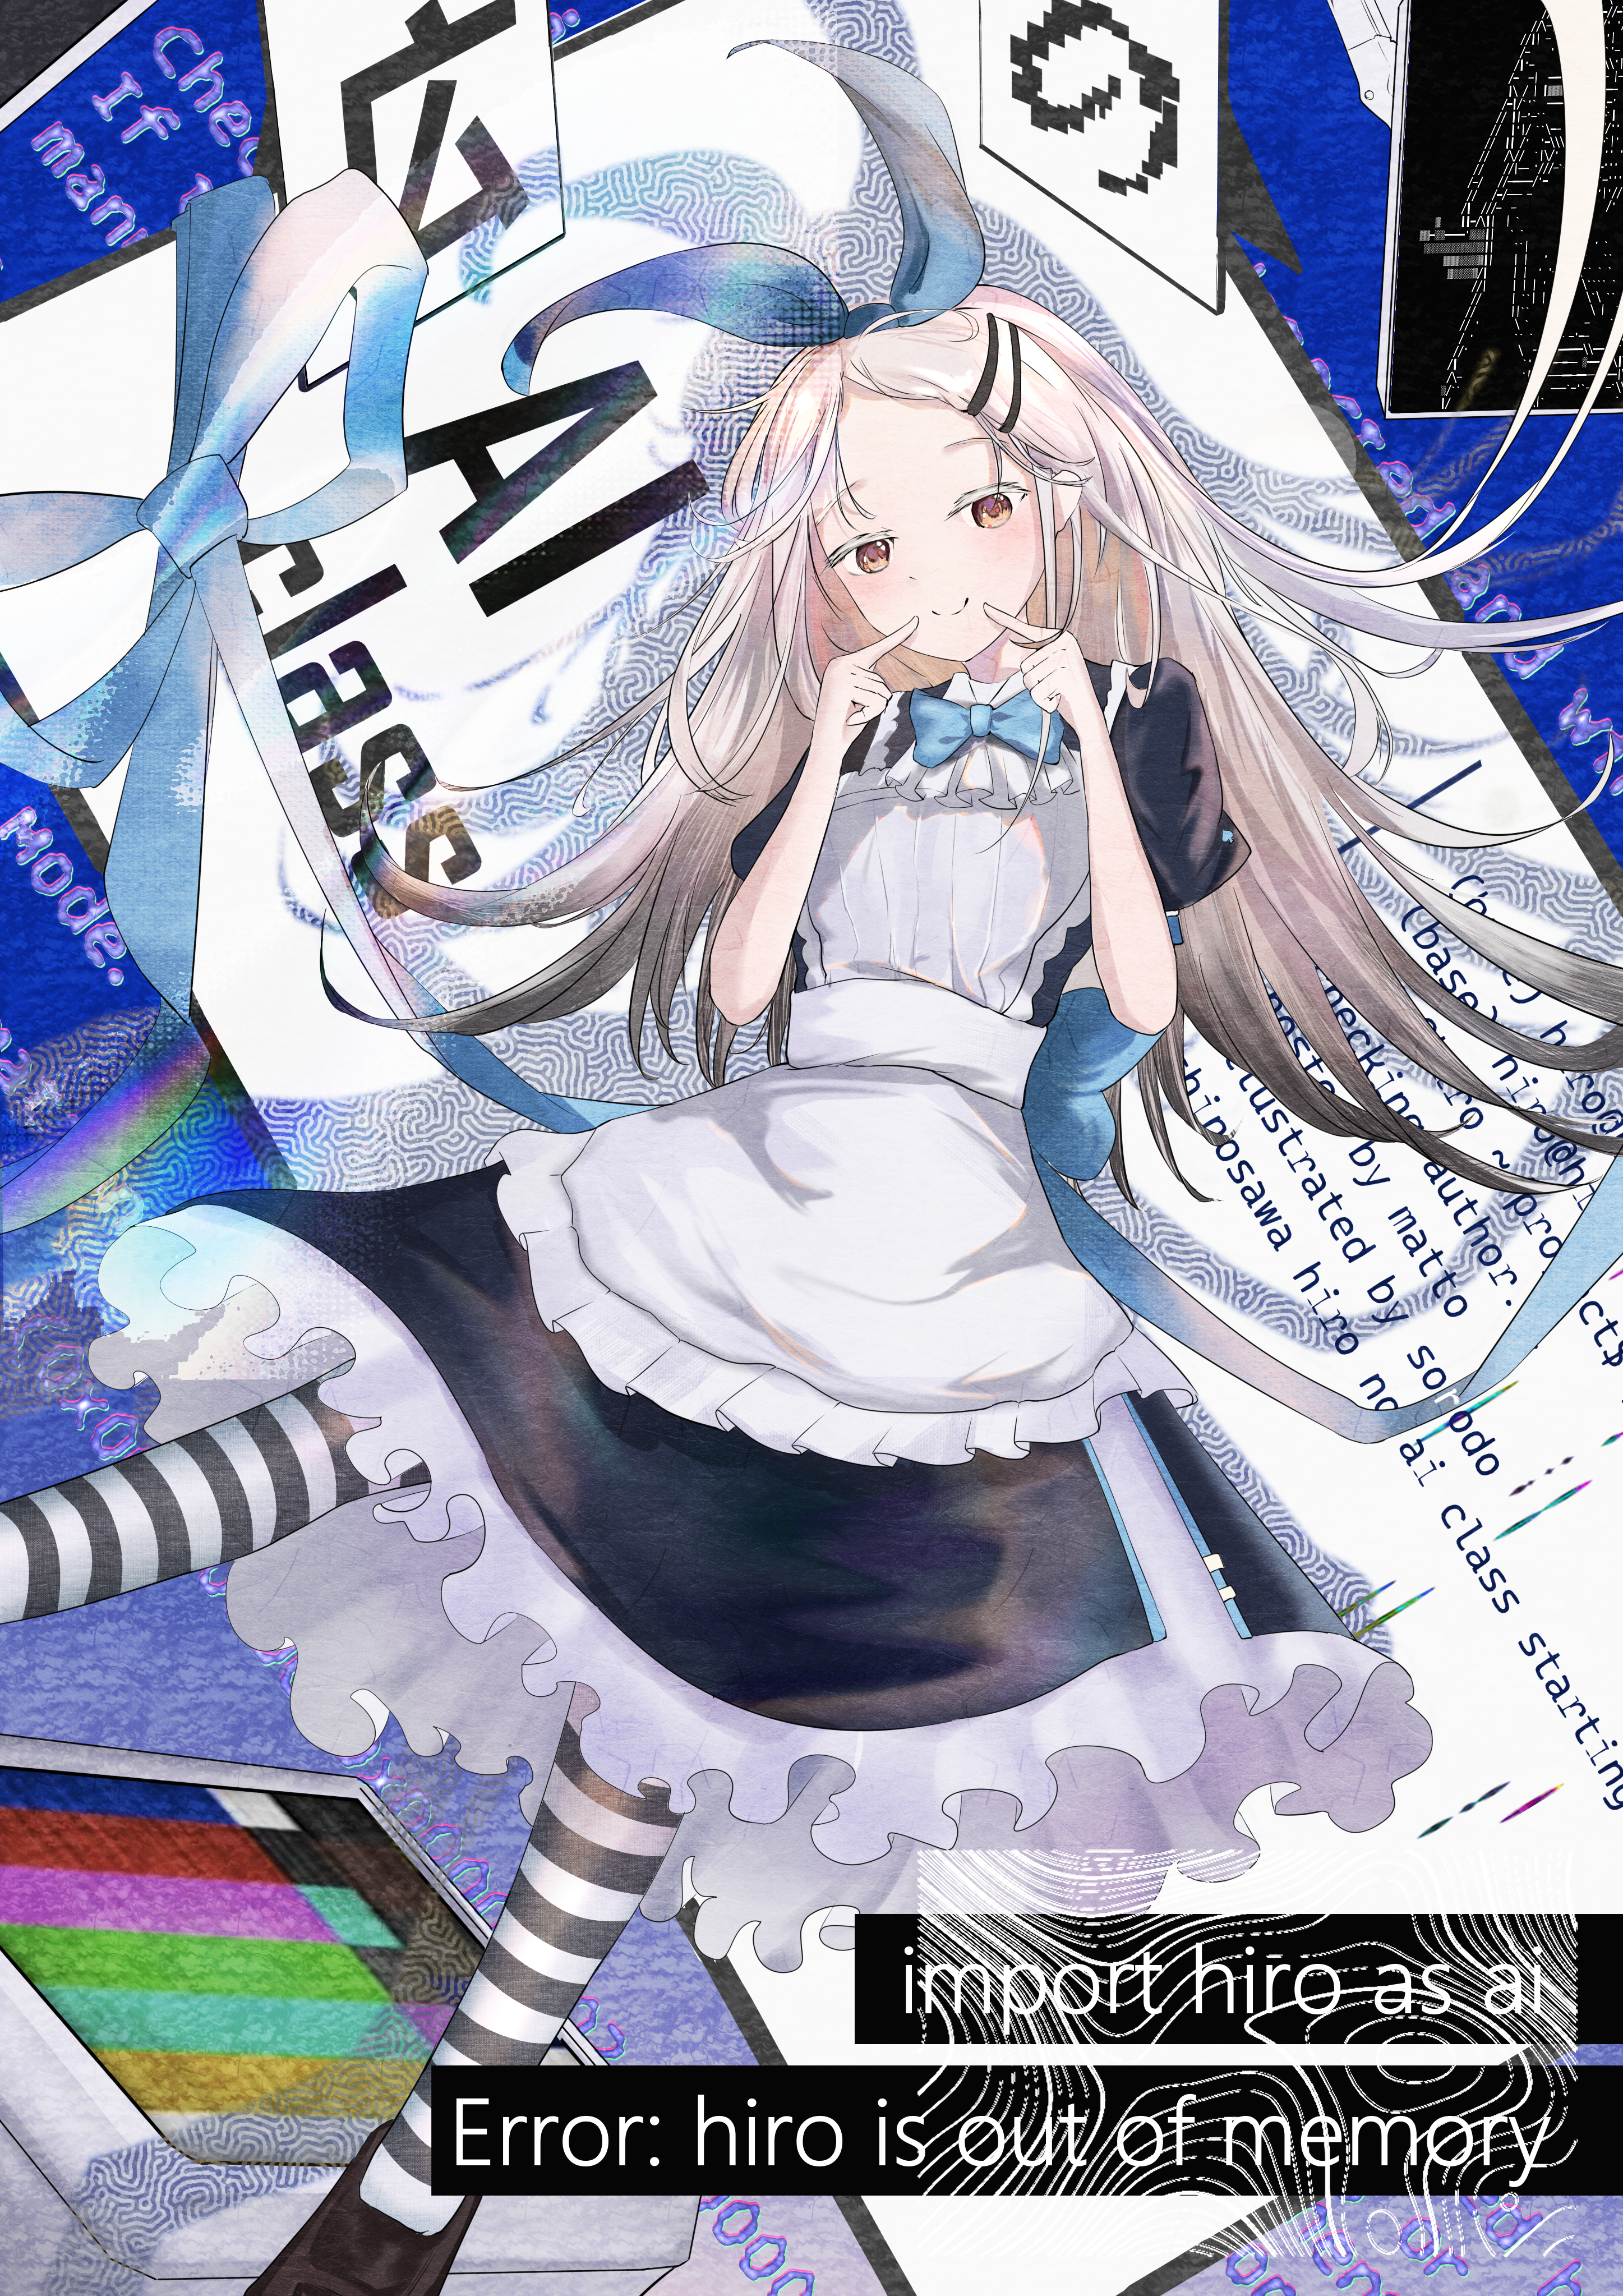
\includegraphics[width=\paperwidth,height=\paperheight,keepaspectratio]{figures/hiroAIbook.png}};
\end{tikzpicture}}
\clearpage

% --- 前言 ---
\frontmatter
\hirotoc
% ==================== 前言 ====================
\chapter*{前言}
\phantomsection
\addcontentsline{toc}{chapter}{前言}

在这里写前言内容。


% --- 正文 ---
\mainmatter

% ==================== 章节1：深夜小茶会 ====================
\chapter{深夜小茶会}

% --- 小剧场 ---
\section*{初星学园——11:40P.M. 活动室}
\phantomsection
\addcontentsline{toc}{section}{小剧场}

\skitillustration{figures/skits/ch01-night-tea.png}

深夜的活动室只剩一盏灯。窗外的初星学园安静得像被谁按下暂停键。

Producer 在桌边收训练记录，笔尖划过纸面。広抱着热茶，坐在旁边，看起来像快睡着了，又像正在读取什么很长的日志。

P：今天先到这里。你已经很累了。

広：嗯。身体的电量，确实很低。

P：你还知道。

広：知道。不代表会停止观察。

Producer 叹了口气，把最后一页记录夹进文件夹。

P：如果有个小助手就好了。至少能在你倒下以后，把后面的事接着做完。

広抬起眼。

P：我只是随口说。

広：随口说出来的愿望，也可以成为需求。

第二天，広把一张手写纸放到桌上。标题写得很认真：

\begin{center}
小広计划：第一版需求草案
\end{center}

下面分着“目标”“限制”“失败条件”“暂不考虑事项”。字很小，结构却清楚得像正式项目文档。

P：你真的写了？

広：嗯。你昨天说出口了。

P：这里为什么有一条“本体容易倒下”？

広：系统风险。

P：这行划掉。

広把纸往自己这边轻轻拉了一点。

広：不可以。风险不能因为看起来可怜就消失。

P：你把自己写得像硬件缺陷。

広：硬件缺陷也可以设计边界。这样比较温柔。

Producer 没有立刻反驳。他看着那行字，又看向她手里的热茶。

P：为什么来真的？

広：因为你说出口了。……而且很不适合我。

她停了一下，像是在确认结论。

広：这样很好。

\clearpage

% 正文内容
\section{深夜小茶会}

这本小册子的起点，不是实验室，也不是发布会。

它从一杯快凉掉的热茶开始，从一句本来不该被认真对待的话开始。Producer 以为自己只是在担心広的身体，広却把那句话翻译成一门课题：如果想做一个能把事情继续接下去的“小広”，要先理解 AI 是怎样从文字、计划、身体和失败里一点点长出来的。

所以，后面的每一章都不是单纯的技术讲义。

它们更像放学后的补课记录：有白板，练习室，门把手，胶带，也有一台很慢、很笨、终于把世界往前推了一点的试作机。

% ==================== 章节2：大语言模型的前世今生 ====================

% --- 章节标题页（竖排） ---
\hirochapter{大语言模型的前世今生}

% --- 小剧场对话 ---
\section*{小剧场}
\phantomsection
\addcontentsline{toc}{section}{小剧场}

午后的初星学园很安静。练习室的窗帘被风吹起一点。广站在白板前，看见上一节课没有擦干净的粉痕。

Producer 把马克笔递给她，没有马上松手。

“站得住吗？”

“三分钟。”我看了一眼墙上的钟，“如果中途坐下，就把它当作实验误差。”

“那就两分钟半。”

“嗯。很过分，だ、ね。”

广这样说着，还是接过了笔。

“今天讲大语言模型？”

她点头。接过笔，先没有写标题，而是在白板中央写下一行：

\begin{quote}
给定前面的文字，预测后面会出现什么。
\end{quote}

“只是这样？”

“只是这样。”广说，“所以很有趣。”

她把“预测”两个字圈起来。

“如果预测得很差，就是胡言乱语。如果预测得好一点，就是自动补全。如果预测得非常好，就会像是在回答问题、写文章、解释代码。”

Producer 看着白板：“那它是真的理解了吗？”

广停了一下，指尖扶住白板边缘，确认自己还算站得稳定。

“这个问题太快了。请再准确一点。”

她在白板左边写下“规则”，中间写下“统计”，右边写下“规模”。

“先看它怎么出生。一个东西从很笨，到很有用，中间不一定有某个瞬间突然获得灵魂。很多时候，它只是把同一件事做到了极限附近。”

“预测下一个词？”

“嗯。”

她把马克笔放回笔槽。

“做不到。再预测一次。”

她轻轻笑了一下。

“这里就是今天的课题。”

\clearpage

% --- 课堂讲义正文（IEEE风格，单栏） ---
\hiropapertitle{大语言模型的前世今生}{広}{初星学园}

\begin{abstract}
大语言模型的核心训练目标可以被概括为：给定上下文，预测下一个 token。这个目标很小，却在一次次撞到语言的边界之后，被迫长出新的结构：规则写不完真实语言，统计模型看不远，循环记忆训练太慢，预训练模型会续写却不一定会帮忙，聊天助手会帮忙却不一定可靠，能调用工具以后又必须面对权限、审计与责任。这堂“筱澤広小课堂”沿着这条问题链，结合代表性论文、公开产品节点、少量公式与原创示意图，说明大语言模型如何从“会接话”发展到“能协作”，并讨论它的能力边界、幻觉风险、系统可靠性与 agent 化趋势。
\end{abstract}

\keywords{大语言模型；Transformer；预训练；指令微调；RLHF；RAG；推理模型；AI agent}

\section{太小的起点：预测下一个 token}

如果只看结果，大语言模型很像突然出现的东西。

昨天我们还在搜索框里输入关键词，今天就可以对一个聊天窗口说：“帮我解释这段代码”“把会议纪要整理成待办”“用更温柔的语气改写这封邮件”。它会回答，会追问，会犯错，也会在某些时刻显得异常聪明。

于是问题来了：它到底是什么？

最短的答案是：大语言模型是一种被大规模训练过的概率模型。它阅读上下文，然后预测下一个 token。所谓 token，可以先粗略理解成文字被切成的小片段。一个汉字、一个英文词、一段词根、一个标点，都可能成为 token。

这听起来像文字接龙。可是，文字接龙接到极高水平时，会碰到很多我们原本以为属于“理解”的事情。要接好一句法律解释，它要知道术语关系；要接好一段代码，它要知道语法和运行结果；要接好一封道歉邮件，它要知道语气、责任和人际边界。

所以，广没有急着判断它有没有“真正理解”。她先把问题收窄：

\begin{quote}
为什么预测下一个 token 这件事，可以一路长成今天的大语言模型？
\end{quote}

这不是一条平滑的直线。更像一串很小的失败：规则覆盖不了，于是需要统计；统计看不远，于是需要表示和记忆；记忆会累、训练会慢，于是需要注意力；模型会续写，却不一定听题；模型会听题，却不一定说真话；模型能调用工具以后，又必须被边界约束。

也就是说，这堂课不是把技术名词排成年表。白板上只留下一个问题：

\begin{quote}
每一代方法解决了什么，又把下一个问题暴露在哪里？
\end{quote}

\begin{figure}[htbp]
\centering
\begin{tikzpicture}[>=stealth, every node/.style={font=\small}]
  \node[draw, rounded corners, align=center, text width=2.8cm] (ctx) at (0,0) {上下文\\今天的课题是};
  \node[draw, rounded corners, align=center, text width=2.8cm] (model) at (4,0) {语言模型\\计算概率分布};
  \node[draw, rounded corners, align=center, text width=2.8cm] (next) at (8,0) {下一个 token\\``大''、``AI''、``...''};
  \draw[->] (ctx) -- (model);
  \draw[->] (model) -- (next);
\end{tikzpicture}
\caption{语言模型的最小直觉：读上下文，预测下一个 token。}
\end{figure}

这张图就是课堂的起点。后面的复杂技术，都会回到它身上：怎样表示上下文，怎样计算概率，怎样训练参数，怎样让模型更听人话，怎样让它查资料、用工具、减少胡编。

不过，“预测”这个词本身也容易让人误会。它不是简单地从词典里挑一个最常见的词，也不是像搜索引擎那样把某个网页片段搬出来。更接近的说法是：模型把前文压缩成一组数值表示，再在整个词表上计算一个概率分布。这个分布里，某些 token 的概率高，某些 token 的概率低。生成时，模型根据这个分布选择一个 token，把它接到上下文后面，再重复下一轮。

Producer 举手：“token 是字吗？还是词？”

“都可能。”广说，“也可能是半个词、一个标点，或者一段常见字符。”

tokenizer 会先把原始文本切成模型词表里的小单位。中文里，一个 token 有时像一个字，有时像一个词；英文里，一个 token 可能是完整单词，也可能是词根或后缀。模型真正处理的不是纸面上的“句子”，而是一串 token 编号。编号查表变成向量，向量经过很多层计算，最后再变成下一个 token 的概率。

她在“切分”下面画了一条线。

“第一步不是理解。”

“第一步是把文字变成机器能计算的颗粒。”

所以，一次回答其实是一串很多小决定。每个 token 都只是一步，几百上千步连起来，才变成一段解释、一封邮件或一段代码。也正因为它是一步一步生成的，前面一步的小偏差会影响后面的路线。模型看起来是在“一口气回答”，内部却更像在一格一格铺路。

这也是为什么同一个问题有时会得到不同答案。模型并不是只保存了一个唯一答案，而是在一个概率空间里行动。温度、采样策略、上下文细节，都会改变它最后走到哪里。先理解这一点，后面的“幻觉”“推理”“工具调用”才不会显得神秘。

广把这里讲得很慢。

“先不要把它想成会说话的人。”

她停了一下，把马克笔换到左手，补上第二句。

“先把它想成一台非常认真、非常庞大的预测机器。”

\subsection*{数学骨架：把“接话”写成概率}

论文里讲语言模型，通常不会从“会聊天”开始，而是从一个概率分解开始。假设一段文本被切成 token 序列：

\[
x_1,x_2,\ldots,x_T
\]

语言模型要估计整段文本出现的概率。按照链式法则，可以写成：

\[
P(x_{1:T})=\prod_{t=1}^{T}P(x_t\mid x_{<t})
\]

这里的 \(x_{<t}\) 表示第 \(t\) 个 token 之前的所有 token。也就是说，模型并不是一次性吐出整篇文章，而是在每个位置上问自己：已经看到前面这些内容，下一个 token 应该是什么？

训练时，模型会在大量文本上反复猜答案。猜错了，就调整参数。常见的训练目标可以写成负对数似然：

\[
\mathcal{L}=-\sum_{t=1}^{T}\log P(x_t\mid x_{<t})
\]

这个式子不用吓人。它的意思很朴素：真实答案出现时，模型给它的概率越高，损失越小；模型越不相信真实答案，损失越大。训练就是让这个损失下降。

Producer 在旁边写下“老师批改”。

“差不多。”广说，“但这里没有老师逐句写评语。答案藏在文本自己里面。”

这就是自监督学习的直觉。对于一段现成文本，前面的 token 可以自动变成题目，真实出现的下一个 token 可以自动变成答案。模型不需要人类给每一句话贴标签，也能构造出海量练习题。它不是被教会“事实是什么”，而是被训练成“在这种上下文后，什么 token 最像会出现”。

模型最后输出的不是一个词，而是一整张候选 token 的分数表。通常会先得到一组 logits，可以粗略理解成“还没有归一化的倾向”。再用 softmax 把它们变成概率：

\[
P_i=\frac{\exp(z_i)}{\sum_j\exp(z_j)}
\]

这里 \(z_i\) 是第 \(i\) 个 token 的 logit，\(P_i\) 是它被选中的概率。softmax 有一个很直观的作用：把所有候选项压成一组总和为 1 的概率。高分 token 会更突出，低分 token 不会完全消失。

她用笔帽轻轻点了点分母。

“大家都在里面。只是有的声音比较大。”

Producer 问：“所以不是选一个绝对正确的词？”

“嗯。是先给所有可能性排队。然后，让其中一个走出来。”

这就解释了一个常见现象：模型既有稳定性，也有随机性。对于“法国的首都是”这种上下文，正确 token 的概率会非常集中；对于“请写一个有初星学园味道的开场”，合理续写可能有很多种，概率分布就会更分散。技术上这只是概率分布的形状；落到使用者眼里，就变成了“模型有时很确定，有时很有创意”。

Bengio 等人在神经概率语言模型中已经把“预测下一个词”与分布式词表示结合起来\cite{ch02bengio2003}。后来的 Transformer、GPT 和聊天助手都没有离开这条骨架；它们真正改变的，是上下文怎样表示、参数怎样训练、输出怎样被约束，以及模型怎样接触外部世界。

广把“预测”两个字又圈了一遍。

过去的软件常常需要人先选择功能：翻译按钮、摘要按钮、问答按钮。语言模型则把许多任务都改写成“接下来应该出现什么文本”。翻译是接出另一种语言，摘要是接出压缩版，代码解释是接出自然语言说明。

这也是为什么论文里常说它是 self-supervised learning。训练数据不需要人工逐条标注“这句话的类别是什么”。互联网规模的文本因此变成了巨大的练习册。它不是老师一题一题批改出来的，而是从人类留下的文字痕迹里自己构造题目。

当然，这种训练方式有代价。它学到的是“文本中经常怎样说”，不是“世界事实上怎样运转”。如果许多文本把某个错误说法重复很多遍，模型也可能学进去。如果训练数据里缺少某个小众领域，模型对它的把握就会薄。语言模型的数学目标很漂亮，但它和真实世界之间仍然隔着数据、语境和验证。

这就是它后来能成为通用接口的原因。

她在白板边写下一句话：

\begin{quote}
同一个训练目标，覆盖了很多任务的入口。
\end{quote}

很简单。

也很过分。

不过，把目标写成概率，只是给问题画出骨架。语言本身不会因此变简单。下一步要问的是：如果人想直接把语言规则写进机器里，为什么很快就会失败？

\section{语言太难：规则写不完，统计看不远}

大语言模型的“前世”并不是一开始就有神经网络。

早期聊天程序 ELIZA 是一个很好的入口。Weizenbaum 在 1966 年发表 ELIZA 论文时，展示了一个可以和人进行自然语言交流的程序\cite{ch02weizenbaum1966}。它最著名的 DOCTOR 脚本会模拟心理咨询式对话：用户说“我很难过”，程序可能把句子改写成“你为什么觉得自己很难过？”

这不是现代意义上的理解。它主要依赖模式匹配和替换规则。

所谓模式匹配，就是先在输入里找某种句式，再把句子的一部分填进预先写好的模板里。用户说“我觉得 X”，程序不需要知道 \(X\) 具体意味着什么，只要把它抽出来，套进“为什么觉得 X？”这样的回答里。规则系统的聪明，来自人事先写好的脚本；系统本身并不会从大量对话中更新自己的语言习惯。

Producer 问：“那 ELIZA 和现在的聊天模型，都是在装懂？”

“装懂这个词太快了。”广说，“ELIZA 是规则像懂。大语言模型是统计结构像懂。像的原因不同，危险也不同。”

\begin{figure}[htbp]
\centering
\begin{tikzpicture}[>=stealth, every node/.style={font=\small}]
  \node[draw, rounded corners, align=center, text width=2.6cm] (input) at (0,0) {用户输入\\我觉得 X};
  \node[draw, rounded corners, align=center, text width=2.8cm] (rule) at (4,0) {规则表\\匹配 ``我觉得''};
  \node[draw, rounded corners, align=center, text width=2.8cm] (output) at (8,0) {模板输出\\为什么觉得 X?};
  \draw[->] (input) -- (rule);
  \draw[->] (rule) -- (output);
\end{tikzpicture}
\caption{规则系统的直觉：先匹配句式，再套用模板。}
\end{figure}

它像一个背了很多反问句的人。接话很顺，但没有在心里形成世界模型。可是 ELIZA 的重要性正在这里：它很早就让人看到，只要语言表面足够像理解，人类就可能把理解投射上去。

这件事对今天仍然有提醒意义。很多人第一次和大语言模型聊天时，也会因为它的礼貌、连贯和自信而产生“它懂我”的感觉。ELIZA 时代靠规则制造这种错觉，今天靠大规模统计结构制造更强的错觉。机制不同，人的心理反应却有连续性。

规则系统的问题也很清楚。语言太柔软，场景太多，人又喜欢省略、反讽、打错字。规则写得少，覆盖不了；规则写得多，维护困难，还容易互相冲突。

例如“没关系”三个字，写进规则表时看起来很简单。可是在不同场景里，它可能表示真的原谅，也可能表示压抑不满，也可能只是礼貌结束话题。规则系统必须提前知道场景、语气、关系、前文。只靠句式匹配，很难判断这些看不见的东西。

后来统计语言模型开始接过接力棒。一个经典近似是 n-gram：

\[
P(w_t\mid w_{<t})\approx P(w_t\mid w_{t-n+1},\ldots,w_{t-1})
\]

意思是：预测当前词时，不看全部前文，只看前面 \(n-1\) 个词。这样问题变得可计算，也能从大语料里统计频率。n-gram 的 \(n\) 指的是连续 \(n\) 个词组成的片段；bi-gram 看两个词，tri-gram 看三个词。它不理解句子，只数“这种前缀后面，历史上常接什么”。

如果 \(n=2\)，模型只看前一个词；如果 \(n=3\)，就看前两个词。比如“语言 模型”后面常常接“可以”“训练”“生成”，模型就会给这些词更高概率。这个思路非常朴素，却把语言处理从手写规则推进到了数据驱动：我们不必把所有语法都写出来，可以让语料告诉机器哪些组合常见。

Producer 看着公式：“那只要把 \(n\) 变得很大，不就解决了？”

“看起来是这样。”广点头，“但是词表会膨胀，组合会爆炸，没见过的组合会越来越多。”

但短窗口有短窗口的命运。它看不远。

比如这句话：

\begin{quote}
那本放在图书馆最里面、封面已经褪色、被我拿来压住讲义的书，终于被 Producer 找到了。
\end{quote}

“找到”的对象是很早出现的“书”。如果模型只看前几个词，它很容易迷路。Bengio 等人指出，传统统计模型还会遇到维度灾难：词组合太多，很多合理句子在训练数据里根本没出现过\cite{ch02bengio2003}。

这叫数据稀疏。语言的组合太多了，哪怕语料很大，也不可能覆盖所有句子。一个人从没听过“我把训练记录夹在植物图鉴里”这句话，也能理解它；但如果统计模型完全依赖出现次数，这种新组合就会很难处理。它需要某种泛化能力：知道“训练记录”和“笔记”相近，“夹在书里”和“放进书页”相近，即使原句没出现过，也能推断它的合理性。

于是问题变成了：能不能不要把每个词都当作孤立符号？

能不能让词语之间拥有可学习的距离？

\subsection*{词不是孤岛：从统计频率到连续表示}

词向量的想法，是把词从离散编号变成连续空间里的点。

“猫”“狗”“动物”会因为上下文相似而靠近；“国王”“王后”“男人”“女人”之间可能形成某种方向关系。Mikolov 等人的 word2vec 工作让这种直觉变得非常有影响力：它用高效架构从大规模语料中学习连续词表示，并在词相似度与语法语义关系上取得很强效果\cite{ch02mikolov2013}。

这背后有一个很重要的语言学直觉：词的意义可以从它出现的邻居里看出来。一个词如果经常和“训练”“舞台”“出汗”“节拍”一起出现，它就会被拉向偶像活动和身体练习的语境；一个词如果经常和“参数”“损失”“梯度”一起出现，它就会被拉向机器学习的语境。模型没有读词典，却从上下文里学到词的用法。

在神经网络里，词向量通常来自一个嵌入矩阵。词表里每个 token 对应一行向量。输入 token 之后，模型先查表得到向量，再把向量送入后续网络。这样，“猫”和“狗”不再只是两个互不相干的编号，而是两个可以比较距离、相似度和方向的点。

Producer 问：“所以向量就是给词换了一个编号？”

“不是。”广说，“编号只负责区分。向量还负责靠近和远离。”

如果“猫”和“狗”只是编号 1357 和 2468，模型不知道它们有什么关系。词向量把它们放进连续空间里，相似词会因为上下文相似而靠近。这样，模型遇到训练集中没见过的新组合时，也可以借助相近词的经验做一点泛化。它不再只背“出现过的词串”，而是开始学习词和词之间的可计算关系。

衡量两个词向量相似，常用余弦相似度：

\[
\cos(v_a,v_b)=\frac{v_a\cdot v_b}{\|v_a\|\|v_b\|}
\]

如果两个向量方向接近，余弦值就高。你可以把它想成：两个词是否经常出现在相似语境里。

\begin{figure}[htbp]
\centering
\begin{tikzpicture}[>=stealth, every node/.style={font=\small}]
  \draw[->] (-0.2,0) -- (7.2,0) node[right] {维度 1};
  \draw[->] (0,-0.2) -- (0,3.6) node[above] {维度 2};
  \node[circle, fill=accent, inner sep=2pt, label=above:{猫}] at (1.4,2.4) {};
  \node[circle, fill=accent, inner sep=2pt, label=right:{狗}] at (2.0,2.1) {};
  \node[circle, fill=accent, inner sep=2pt, label=above:{动物}] at (1.7,3.0) {};
  \node[circle, fill=primary, inner sep=2pt, label=above:{代码}] at (5.2,1.1) {};
  \node[circle, fill=primary, inner sep=2pt, label=right:{函数}] at (5.8,1.5) {};
  \node[circle, fill=primary, inner sep=2pt, label=below:{编译}] at (4.8,0.6) {};
\end{tikzpicture}
\caption{词向量的直觉示意：语境相似的词，在空间中更接近。}
\end{figure}

\section{模型长出身体：注意力、预训练与规模}

词向量解决了“词不是孤岛”的问题，但文本还有顺序。句子不是一袋词，而是一条时间线。

“Producer 批评了我”和“我批评了 Producer”用到几乎同一批词，但意思完全不同。词向量能表示词的关系，却不能单独解决顺序和句法。模型还需要知道谁在前，谁在后，哪个修饰哪个，哪个动作指向哪个对象。

循环神经网络尝试按顺序读文本。一个非常简化的状态更新可以写成：

\[
h_t=f(Wx_t+Uh_{t-1})
\]

这里 \(h_t\) 是读到第 \(t\) 个位置时的隐藏状态。它既看当前输入 \(x_t\)，也看上一步的记忆 \(h_{t-1}\)。LSTM 则进一步引入门控机制，试图缓解普通循环网络在长序列里容易遗忘的问题\cite{ch02lstm1997}。

LSTM 的“门”可以粗略理解成三个决定：哪些旧信息要留下，哪些新信息要写入，哪些状态要输出。它比普通 RNN 更像一个会整理笔记的人，不是每读一个词就把所有信息混在一起，而是尝试决定什么值得记住。

这一段可以很短，因为 RNN 不是终点。它的贡献，是把“顺序读”和“带着记忆读”变成了神经网络里的自然操作；它的限制，也正来自这里。它必须一步一步读，不能轻易跳过时间线。

这像边读边做笔记。问题是，笔记本越传越厚，训练越慢；句子越长，早期信息越难稳定保留。模型想记住前文，但前文隔得太远时，它还是会累。

更麻烦的是，循环结构天然按时间一步一步计算。第 \(t\) 步必须等第 \(t-1\) 步算完。对于短句，这还可以接受；对于互联网规模的文本训练，这会成为巨大瓶颈。模型不只是要会记忆，还要能被成千上万张计算卡高效训练。

广说：

\begin{quote}
会累不是失败。\\
是结构在告诉我们，下一步该换方法了。
\end{quote}

说完以后，广发现它很像训练记录，也很像模型史。

\subsection*{注意力成为骨架：让每个位置看向别处}

2017 年，Vaswani 等人发表 \textit{Attention Is All You Need}，提出 Transformer 架构\cite{ch02vaswani2017}。这篇论文的关键主张很大胆：处理序列不一定要依赖循环结构，也不一定要依赖卷积；注意力机制本身就可以成为核心骨架。

注意力的基本公式是：

\[
\mathrm{Attention}(Q,K,V)=
\mathrm{softmax}\left(\frac{QK^T}{\sqrt{d_k}}\right)V
\]

公式里有三个角色：Query、Key、Value。可以把 Query 理解成“我现在在找什么”，Key 是“每个位置提供的索引”，Value 是“真正要取出的信息”。模型用 \(QK^T\) 计算当前位置和其他位置的相关程度，再用 softmax 变成权重，最后加权汇总 Value。

在实现上，\(Q,K,V\) 通常都来自同一批输入向量，只是经过不同线性变换：

\[
Q=XW_Q,\quad K=XW_K,\quad V=XW_V
\]

这里没有人手工规定“主语应该看谓语”或“代词应该看名词”。模型要在训练中自己学会：哪些位置之间互相有用。不同层、不同注意力头会形成不同观察方式：有的头关注相邻词，有的头关注标点，有的头追踪长距离指代。

Producer 把“注意力”圈起来：“这是不是就等于理解？”

“不等于。”广说，“注意力只是计算关联的一种方法。它让位置之间更容易交换信息，不保证交换出来的东西一定正确。”

self-attention 的重点在 self：同一段序列里的 token 彼此计算相关性。每个位置都可以形成自己的 Query，去和其他位置的 Key 比较，再按权重汇总 Value。这样，模型不必像 RNN 那样把前文压进一条递推状态，而是可以在一层计算里让许多位置直接建立联系。

这听起来抽象。换成课堂比喻就简单一点。

老师问：“这句话里的‘它’指什么？”

学生不能只盯着“它”这个字。需要回头看前文：是“语言模型”，还是“训练数据”，还是“注意力机制”？注意力就是让模型在不同位置之间分配目光。

\begin{figure}[htbp]
\centering
\begin{tikzpicture}[every node/.style={font=\small}]
  \node at (0,2.6) {查询词：它};
  \foreach \x/\word/\shade in {0/模型/30,1.6/读过/10,3.2/很多/15,4.8/文本/45,6.4/所以/8,8.0/它/80} {
    \node[draw, fill=accent!\shade, minimum width=1.1cm, minimum height=0.65cm] at (\x,1.4) {\word};
  }
  \node[align=center, text width=7.8cm] at (4,0.25) {颜色越深，表示当前 token 对该位置分配的注意力越高。};
\end{tikzpicture}
\caption{注意力热力图的简化示意。真实模型会在多层、多头中学习更复杂的关系。}
\end{figure}

Transformer 还需要位置编码。因为它不按 RNN 那样一步一步读，所以必须把位置信息注入 token 表示里。原论文使用正弦、余弦位置编码，让模型知道“这个 token 在第几个位置”\cite{ch02vaswani2017}。

它适合大规模训练，原因有三个。

第一，注意力可以直接建立远距离联系。第二，它比循环结构更容易并行计算。第三，多层堆叠后，模型可以逐层组合局部和全局信息。

这里还要加一个边界。Transformer 不是永远让所有 token 随便互看。BERT 这类编码器模型通常可以同时看左右文；GPT 这类自回归生成模型会使用 causal mask，让当前位置不能看到未来 token。也就是说，它能在允许的范围内直接看向别的位置，但生成时仍然要遵守“从左到右”的时间方向。

“多头注意力”也值得多说一句。单个注意力头像一束视线，多头注意力则像从多个角度同时看同一句话。一个头看语法关系，一个头看主题词，一个头看引用对象，一个头看格式边界。它们的结果拼接起来，再经过前馈网络处理。这样，模型不是用一种目光理解文本，而是用许多目光同时扫描。

广把四支不同颜色的笔并排放在桌上。

“同一句话，可以有很多种看法。”

她看向 Producer。

“你看我走路，会看步幅。看呼吸。看脸色。看我是不是在说谎。”

“你经常在说‘没事’的时候说谎。”

“嗯。所以需要多头注意力。”

这也是 Transformer 和早期模型气质不同的地方。RNN 像一个人沿着走廊一步步走，边走边记；Transformer 像把整段话摊在桌上，让每个词在规则允许的范围内直接看向其他词。对于长文本和大规模训练，这种结构上的变化非常关键。

这就是现代大语言模型真正的转折点。

不是因为它第一次会说话，而是因为它终于拥有了一副可以被放大的身体。

\subsection*{预训练：先读很多书}

Transformer 之后，预训练成为主线。

BERT 代表一种理解型路线。它使用双向 Transformer，从左右两侧上下文中学习语言表示。论文强调，BERT 可以在无标注文本上预训练，然后只加很少的任务层，就在问答、自然语言推理等多种任务上取得强效果\cite{ch02bert2018}。

可以把 BERT 想成做完形填空的学生：

\begin{quote}
白板上写着 [MASK]。
\end{quote}

模型要根据左右文判断，遮住的词可能是什么。它擅长理解句子内部关系。

BERT 的代表性任务叫 masked language modeling：把输入里一部分 token 遮住，让模型根据左右文恢复它。因为它做题时能同时看前后，所以很适合给整段文本做判断、匹配、分类和抽取。

Producer 问：“那它不能写文章吗？”

“不是完全不能。”广说，“只是它出生时练的题型，不是从左到右续写。”

GPT 路线更偏生成。GPT-2 和 GPT-3 使用自回归语言建模：只看左边上下文，从左到右生成后续 token\cite{ch02gpt22019,ch02gpt32020}。自回归的意思是，模型把自己刚生成的 token 也放回上下文里，再预测下一个。它像一边走一边铺轨道：前一步写出来的东西，会变成下一步的条件。

这两条路线的差别，不是好坏之分，而是训练目标不同。BERT 在预训练时能同时看左边和右边，所以特别适合做分类、匹配、抽取式问答等“读懂整段文本再判断”的任务。GPT 在生成时只能看左边，所以天然适合继续写：它每一步都只需要回答“接下来是什么”。

后来聊天式大模型大多沿着 GPT 式生成路线发展。原因很实际：对话、写作、代码、计划，最后都要生成一串新 token。理解当然重要，但它被包进生成过程里。模型必须先从上下文里读出任务，再继续写出合适输出。

\begin{figure}[htbp]
\centering
\begin{tikzpicture}[>=stealth, every node/.style={font=\small}]
  \node[draw, rounded corners, align=center, text width=3.2cm] (bert) at (0,0) {BERT\\看左右文\\填空理解};
  \node[draw, rounded corners, align=center, text width=3.2cm] (gpt) at (5.2,0) {GPT\\看左文\\继续生成};
  \node[align=center, text width=3.3cm] at (0,-1.4) {白板上 [MASK]};
  \node[align=center, text width=3.3cm] at (5.2,-1.4) {白板上 → 写下};
\end{tikzpicture}
\caption{BERT 与 GPT 的直觉差异：一个偏填空理解，一个偏顺序生成。}
\end{figure}

预训练的意义，是让模型先在大量文本中学到通用语言规律，再迁移到具体任务。过去很多 NLP 系统要为每个任务单独设计结构；预训练模型则把大量知识和语言模式压进参数里。

这里的“知识”要打引号。它不是数据库里的整齐条目，而是从文本分布中学到的关联。模型知道很多事情，是因为相关表述在训练数据中反复出现；它也会混淆很多事情，因为文本本身有噪声、矛盾和过时信息。

预训练还有一个重要后果：模型内部没有清晰的“知识出处”。人类读书时可以说“我在某本书第几章看到过”，数据库可以返回某条记录，预训练模型却只是把大量文本压进参数。它回答问题时，不是在翻开某一页，而是在参数空间里生成一个看起来合理的延续。这一点会在后面的 RAG 部分变得很重要。

广把预训练称作“漫长的旁听”。

没有老师逐题讲解。

只是坐在那里，听了非常多句子。

嗯。

很像我旁听体能课。

脑子懂了。

身体还没有。

“听得太久，也会累吧？”Producer 问。

“会。”广说，“但是累不一定不好。说明容量正在被使用。”

\subsection*{上下文里学任务：规模带来的临场适应}

GPT-3 的重要性，不只在于参数大。它更醒目的地方，是把 few-shot learning 变成了大语言模型时代的标志性能力\cite{ch02gpt32020}。

所谓 few-shot，就是不用重新训练模型，只在提示词里给几个例子。比如：

\begin{quote}
中文：早上好。\\
日文：おはよう。\\
中文：谢谢。\\
日文：ありがとう。\\
中文：今天的训练很难。\\
日文：
\end{quote}

模型看到这种格式，就会继续补出对应答案。它没有为“这个翻译任务”单独更新参数，而是在上下文里识别任务模式。

这件事后来被称作 in-context learning。它像一种临场适应：参数不变，但上下文改变了模型当前的行为。你给它三个翻译例子，它就进入翻译模式；你给它几条 JSON 样例，它就尝试继续生成 JSON；你给它一段角色设定，它就调整语气和词汇。

这也是提示词为什么重要。提示词不是对模型“下命令”这么简单，它更像临时搭了一个小环境。环境里有规则、示例、格式、限制和语气。模型根据这个环境继续生成。环境越清楚，模型越容易落到正确轨道；环境越含糊，它就越可能走偏。

Producer 问：“所以 prompt engineering 是给模型写说明书？”

“不只是说明书。”广说，“更像布置考场。”

说明书告诉它要做什么，例子告诉它题型是什么，格式告诉它答案长什么样，角色和语气告诉它要站在哪里说话。强模型会从这些上下文线索里推断当前任务。弱模型也会照着格式走，但可能只学到表面。

\begin{figure}[htbp]
\centering
\begin{tikzpicture}[>=stealth, every node/.style={font=\small}]
  \node[draw, rounded corners, align=center, text width=2.1cm] (ex1) at (0,0) {示例 1\\输入→输出};
  \node[draw, rounded corners, align=center, text width=2.1cm] (ex2) at (2.8,0) {示例 2\\输入→输出};
  \node[draw, rounded corners, align=center, text width=2.1cm] (q) at (5.6,0) {新问题\\输入→?};
  \node[draw, rounded corners, align=center, text width=2.1cm] (a) at (8.4,0) {模型续写\\输出};
  \draw[->] (ex1) -- (ex2);
  \draw[->] (ex2) -- (q);
  \draw[->] (q) -- (a);
\end{tikzpicture}
\caption{少样本学习的直觉：任务说明和例子直接放进上下文。}
\end{figure}

这件事很像临时看题型。老师没有重新训练学生的大脑，只是在卷面上给了两道样题。足够强的学生会看出格式，然后照着做第三题。

GPT-3 论文同时也很谨慎。它指出模型在一些任务上仍然挣扎，也讨论了大规模网页语料带来的方法问题和社会影响\cite{ch02gpt32020}。这很重要：大，不等于稳；会举一反三，不等于每次都对。

few-shot 的能力尤其容易让人高估模型。因为它看起来像“读懂了新任务”。但很多时候，它是在捕捉格式、词面线索和相似任务模式。简单任务上这足够好，复杂任务里就可能露出问题：题目条件稍微变形，示例带有误导，输出格式和事实正确性同时受约束，模型就可能只学到了表面形式。

所以，这一节的结论不是“模型突然会思考了”。

更准确的说法是：当模型足够大、训练足够广，它开始能把上下文本身当作任务说明。

广说：“它不是读懂了考试制度。”

“它只是很会看题面。”

这里还欠一个问题：为什么“足够大、训练足够广”会带来这种临场适应？它不是魔法，而是规模、数据和计算共同把损失压低以后，许多语言模式开始在同一个模型里相互借力。

\subsection*{规模律：大，不只是参数大}

为什么大模型会变强？业界论文里有一条重要线索叫 scaling laws。

Kaplan 等人的工作发现，语言模型损失会随着模型规模、数据规模和训练计算量呈现较规律的幂律下降趋势\cite{ch02scaling2020}。简化地说，可以写成一种直觉形式：

\[
L(N,D,C)\downarrow
\quad\mathrm{when}\quad
N,D,C\uparrow
\]

其中 \(N\) 是参数量，\(D\) 是训练数据量，\(C\) 是计算量。实际论文里的拟合更细，但科普时抓住这个方向就够：变大通常会带来更低损失、更强能力。

这里的“损失下降”不是一个抽象数字。它意味着模型在预测下一个 token 时更少惊讶。很多能力就是从这种“不那么惊讶”里浮出来的：它更熟悉代码结构，更熟悉论文写法，更熟悉多轮对话，更熟悉人类如何一步步解释问题。

可是，如果只记住“越大越好”，就会误读这条线。

Chinchilla 论文进一步指出，在固定计算预算下，很多大语言模型其实是“训练不足”的：参数很多，但数据不够。它建议模型参数量和训练 token 数应当更均衡地增长，并展示了 70B 参数的 Chinchilla 在相同计算预算下击败更大模型的结果\cite{ch02chinchilla2022}。

\begin{figure}[htbp]
\centering
\begin{tikzpicture}[>=stealth, every node/.style={font=\small}]
  \draw[->] (0,0) -- (7.4,0) node[right] {参数量 \(N\)};
  \draw[->] (0,0) -- (0,3.6) node[above] {训练数据 \(D\)};
  \draw[thick, color=accent] (0.7,0.6) -- (6.4,3.1);
  \node[align=center, text width=2.5cm] at (4.9,2.1) {较均衡\\训练更充分};
  \node[draw, rounded corners, align=center, text width=2.3cm] at (5.2,0.8) {参数大\\数据不足};
  \node[draw, rounded corners, align=center, text width=2.3cm] at (1.6,2.8) {数据多\\模型太小};
\end{tikzpicture}
\caption{Chinchilla 式直觉：固定预算下，模型大小和训练数据要匹配。}
\end{figure}

LLaMA 的思路也延续了这种更重视训练效率的方向。它强调用更多 token 训练较小模型，展示了开放权重基础模型可以在较低推理成本下取得很强表现\cite{ch02llama2023}。后来 Llama 3.1 等模型进一步把“开放权重模型也能接近前沿能力”变成产业事实之一\cite{ch02llama312024}。这里说开放权重，而不是简单说开源，是因为模型权重、训练数据、训练代码和使用许可的开放程度并不总是相同。

这对产业也很关键。一个最大、最贵的模型可能在榜单上最好，但真实应用还要考虑延迟、成本、隐私、部署环境和可控性。客服系统、手机输入法、企业知识库、嵌入式设备，不一定都需要最大模型。它们需要的是在目标任务上足够好、足够快、足够便宜、足够安全。

Producer 问：“那模型越小越好吗？”

“也不是。”广说，“只是问题变成了匹配。”

大模型像总科室，见多识广，但贵、慢、部署难；小模型像专门训练过的值日生，在固定场景里可能更快、更稳、更便宜。规模律讲的是趋势，不是替你做产品决策。真正的问题是：任务需要多少能力，数据能不能支撑，预算和延迟能不能接受。

因此，规模不是单一旋钮。它像训练菜单。

只加重量，不加恢复，会受伤。只加练习量，不提升动作质量，也会卡住。模型也一样：参数、数据、算力、训练配方、评测方式，都在共同决定它最后的能力。

Producer 在旁边把“休息”两个字写得很大。

广看了一眼。

“我知道。”

“你每次都说知道。”

“因为每次都还没学会。嗯，很适合复习。”

嗯。

不是只要变大就好。

要正确地变大。

可是，正确地变大之后，模型仍然只是在续写。它可以看懂题面，却未必知道自己应该认真答题；它可以接出一段像答案的文字，却未必站在用户这一边完成任务。下一道墙，就在这里。

\section{从续写到助手：对齐、幻觉与检索}

原始预训练模型会续写文本，但它不一定会“听话”。

你问它“请解释这段代码”，它可能解释，也可能续写成一篇博客，也可能编造上下文。原因很简单：预训练目标只要求它预测文本分布，没有明确告诉它“用户希望你完成任务”。

InstructGPT 论文把这个问题讲得很清楚：更大的语言模型并不天然更符合用户意图，可能不真实、有害，或者根本不帮忙\cite{ch02instructgpt2022}。他们使用人类反馈进行训练，大致分三步：

\begin{enumerate}
  \item 收集人工示范，用监督学习微调模型。
  \item 收集人类对多个回答的排序，训练奖励模型。
  \item 用强化学习优化模型，让它生成更受人类偏好的回答。
\end{enumerate}

\begin{figure}[htbp]
\centering
\begin{tikzpicture}[>=stealth, every node/.style={font=\small}]
  \node[draw, rounded corners, align=center, text width=2.3cm] (sft) at (0,0) {人工示范\\SFT};
  \node[draw, rounded corners, align=center, text width=2.5cm] (rm) at (3.4,0) {答案排序\\奖励模型};
  \node[draw, rounded corners, align=center, text width=2.5cm] (rl) at (6.9,0) {强化学习\\优化策略};
  \draw[->] (sft) -- (rm);
  \draw[->] (rm) -- (rl);
\end{tikzpicture}
\caption{RLHF 的三阶段直觉：先学示范，再学偏好，最后按偏好优化。}
\end{figure}

一个直觉式的 RLHF 目标可以写成：

\[
\max_\pi \; r_\phi(x,y)-\beta D_{\mathrm{KL}}(\pi(y\mid x)\,\|\,\pi_0(y\mid x))
\]

这里 \(r_\phi\) 表示奖励模型给回答的分数，后面的 KL 项约束新模型不要离原模型太远。实际训练细节会更复杂；这个式子只是抓住一个核心直觉：让模型更接近人类偏好的回答，同时不要偏离原本语言能力太多。

直觉上，它像 Producer 给广安排训练：可以把她推向更好的表现，但不能把人推到完全失控。

“准确的严厉，是训练。”广说。

“没有边界的严厉呢？”

“那只是噪声。没有学习价值。”

这里最容易误解的是“奖励”。奖励模型不是事实裁判，也不是道德本身。它只是从人类偏好数据中学到“哪种回答更像人类标注者喜欢的回答”。如果标注标准好，它会帮助模型更有用、更诚实、更安全；如果标准含糊，模型也可能学会讨好、回避或说得更漂亮。

Producer 问：“那 RLHF 会让模型变真实吗？”

“会改善。”广说，“但不能保证。”

人类偏好可以奖励“承认不知道”，也可以奖励“说话有条理”。可是事实正确性还需要数据、检索、工具、评测和产品约束一起工作。一个回答听起来诚恳，不等于它引用的论文真的存在。对齐让模型更像助手，不让模型自动变成事实数据库。

所以 RLHF 的意义不是让模型获得真理，而是把“续写互联网文本”的模型拉向“回答用户问题”的模型。它把原本开放的文本分布，收束到更符合助手角色的区域：更愿意遵循指令，更少输出危险内容，更常承认不确定。

LaMDA 论文从对话模型角度讨论了质量、安全与事实扎根等指标\cite{ch02lamda2022}。ChatGPT 的发布则把这种指令跟随与对话交互推向大众产品\cite{ch02chatgpt2022}。

对普通使用者来说，这一步比参数量更有体感。一个没有对齐的强模型像非常会写但不听题的学生；一个经过指令微调和人类反馈的模型，才像愿意按照题目作答的助手。ChatGPT 的“产品震感”很大程度来自这里：人第一次可以不写代码、不设计任务头，只用自然语言描述目标，就驱动模型工作。

所以，ChatGPT 不是“语言模型突然会聊天”。它更像一个预训练模型被指令微调、人类反馈和产品化对话界面慢慢推到桌前，终于开始认真听题。

广在白板角落补了一行：

\begin{quote}
它不是变成人。\\
它只是终于知道，题目要求不是“继续写”，而是“帮我做”。
\end{quote}

\subsection*{会帮忙，不等于说真话}

大语言模型最危险的地方，不是它什么都不会。

而是它经常说得很像会。

模型训练目标是生成高概率文本，不是保证事实正确。它可能把真实术语、相似人名、常见论文格式和不存在的细节拼在一起，生成一个看起来很可靠的错误答案。这就是常说的幻觉。

幻觉的麻烦在于，它不是总以“明显错误”的样子出现。低质量答案很容易发现；高质量幻觉反而危险。它可能格式正确，语气稳重，引用看起来像真的，推理过程也很顺。如果只看表达流畅度，很容易被它带走。

解决幻觉不能只靠“让模型更诚实”。很多时候，模型需要外部资料。

RAG，也就是检索增强生成，把语言模型和信息检索结合起来。Lewis 等人的 RAG 工作把参数化生成模型与非参数化记忆结合，在知识密集型任务上取得改进\cite{ch02rag2020}。广在旁边写了更短的说法：不要只凭记忆答题，先查资料，再带着资料回答。

RAG 的价值有两层。第一，它能补充新知识。模型训练完成后，参数里的知识会慢慢过时，而检索系统可以访问更新的文档。第二，它能提供可检查的证据。模型不只是给一个答案，还可以把相关资料片段带出来，让人知道它依据什么回答。

Producer 问：“所以接了 RAG，就不会胡编了？”

“不会。”广说，“只是多了一条能被检查的路。”

RAG 至少有三件事要同时成立。第一，检索器要找对资料；第二，资料片段要真的进入模型上下文；第三，生成答案时要忠实使用这些资料。任何一层出错，最后都可能变成“带着资料胡编”。有时模型找到了正确文档，却引用错段落；有时资料本身过期；有时多个来源互相冲突，模型选择了看起来更顺口的那个。

\begin{figure}[htbp]
\centering
\begin{tikzpicture}[>=stealth, every node/.style={font=\small}]
  \node[draw, rounded corners, align=center, text width=2cm] (q) at (0,0) {问题};
  \node[draw, rounded corners, align=center, text width=2.4cm] (ret) at (2.8,0) {检索器\\找资料};
  \node[draw, rounded corners, align=center, text width=2.5cm] (ctx) at (5.9,0) {上下文\\证据片段};
  \node[draw, rounded corners, align=center, text width=2.2cm] (gen) at (9,0) {模型\\生成回答};
  \draw[->] (q) -- (ret);
  \draw[->] (ret) -- (ctx);
  \draw[->] (ctx) -- (gen);
\end{tikzpicture}
\caption{RAG 的直觉：先找证据，再生成回答。}
\end{figure}

GPT-4 技术报告也反复强调能力评测、安全评估与局限性\cite{ch02gpt42023}。Constitutional AI 则探索用一组原则和 AI 反馈来改进无害性，减少完全依赖人类逐条标注的成本\cite{ch02constitutional2022}。

但 RAG 也不是万能药。检索器可能找错资料，资料本身可能过时，拼进上下文的证据可能被模型误读。更现实的问题是：当证据很多、互相冲突、质量不一时，模型仍然需要判断。可靠系统不能只写“接入 RAG”四个字，还要设计文档清洗、权限控制、引用格式、冲突处理、答案溯源和人工复核。

这一段的重点是：可靠性不是一个按钮。

它需要多层机制：更好的训练数据，更好的对齐，更好的检索，更明确的引用，更严格的评测，以及人在关键场景里的复核。

广在这里停顿了一下。

“它很强。所以更要确认。”

这句话不是保守。

是使用强工具时最基本的礼貌。

她把讲义翻到引用列表那一页。

“资料也会说谎。或者过期。或者只说了一半。”

Producer 点头：“所以要看来源。”

“嗯。プロデューサー也是。”

“我？”

“你说‘今天只练一点’，也需要验证。”

到这里，模型已经从“会接话”走到“会回答”，又被事实和来源拉住。但现实工作不只是问答。很多任务需要查资料、算结果、改文件、操作系统界面。于是，语言模型开始从答案走向行动。

\section{从回答到行动：工具、Agent 与边界}

当模型能稳定对话后，人们很快发现：只让它直接给答案还不够。很多任务需要中间步骤。

Chain-of-Thought 论文提出，在提示中给出推理过程示例，可以显著提升大模型在算术、符号和常识推理任务上的表现\cite{ch02cot2022}。它的直觉很简单：不要只让模型写最终答案，而是让它先把问题拆开。

这里的 chain 不是神秘的大脑链条，而是可见的中间文本。模型先生成“我应该怎样分解问题”，再用这些文字继续生成后面的步骤。对自回归模型来说，前面生成的每一句话都会成为后面预测的上下文。因此，中间步骤写得好，后面更容易落到正确答案；中间步骤写错，也会把错误传下去。

例如：

\begin{quote}
问题：练习室有 3 个水杯，我又拿来 2 个，Producer 收走 1 个，还剩几个？\\
推理：先有 3 个，加 2 个变 5 个，收走 1 个，还剩 4 个。\\
答案：4。
\end{quote}

注意，这不意味着模型真的像人一样在心里思考。它只是生成了中间文本，而这些中间文本会帮助后续 token 更容易落到正确轨道上。

因此，链式思维更像一种外化的草稿纸。对复杂问题，人类也常常需要把步骤写出来。模型生成中间步骤后，后续生成可以引用前面的中间结果，减少一步跳到答案时的压力。不过，草稿纸也可能写错。一步错，后面每一步都可能跟着错。

ReAct 进一步把 reasoning 和 acting 交替起来：模型一边写推理痕迹，一边执行动作，从外部环境获得观察结果\cite{ch02react2022}。Toolformer 则探索让模型学习什么时候调用外部 API、传什么参数、如何把工具返回结果融入后续预测\cite{ch02toolformer2023}。

Producer 问：“只要会调用工具，就是 agent 吗？”

“还不够。”广说，“会拿工具，和会完成任务，中间差很多。”

从这里开始，模型不再只是语言空间里的续写器。它可以把“需要知道今天的天气”转成查询工具，把“要分析这份表格”转成代码执行，把“要安排会议”转成日历操作。语言变成控制层，工具变成手脚。

\begin{figure}[htbp]
\centering
\begin{tikzpicture}[>=stealth, every node/.style={font=\small}]
  \node[draw, rounded corners, align=center, text width=2.3cm] (thought) at (0,0) {Thought\\需要查什么};
  \node[draw, rounded corners, align=center, text width=2.3cm] (action) at (3.5,0) {Action\\调用工具};
  \node[draw, rounded corners, align=center, text width=2.3cm] (obs) at (7,0) {Observation\\得到结果};
  \draw[->] (thought) -- (action);
  \draw[->] (action) -- (obs);
  \draw[->] (obs) to[bend left=35] (thought);
\end{tikzpicture}
\caption{ReAct 式循环：推理、行动、观察交替进行。}
\end{figure}

这就是 AI agent 的雏形：模型不只是回答，还能规划、查资料、调用工具、观察结果、继续修正。

agent 的关键不是“自主”两个字，而是闭环。只生成计划，不观察执行结果，还是纸上谈兵；只调用工具，不会解释目标，也只是自动脚本。真正有用的 agent 要能把目标拆成步骤，在每步之后读取环境反馈，再决定下一步。

当然，这也放大了风险。一个只会写错答案的模型，最多误导你；一个会调用工具的模型，可能发错邮件、删错文件、查错数据。所以 agent 的核心不是“让模型自由行动”，而是给它边界、权限、回滚和审计。

到 2025 年以后，这条路线已经进入产品层。OpenAI 的 Computer-Using Agent 把视觉输入、鼠标键盘操作和网页任务结合起来，说明 agent 不只是调用一个天气 API，也可能直接操作图形界面\cite{ch02cua2025}。这让边界问题更严肃：模型不只是在文本里犯错，而可能在真实软件里点错按钮。

广说：

\begin{quote}
能动起来，不代表可以乱跑。
\end{quote}

プロデューサー 会先确认身体状态。

系统也一样，要先确认安全边界。

\subsection*{已经显形的未来：预测语言碰到世界边缘}

讲义写到这里时，大语言模型的“未来”已经不完全是未来。几条路线正在同时产品化。

先是多模态。模型不只处理文字，也处理图像、音频、视频和结构化数据。GPT-4 技术报告已经展示了更强的综合能力，虽然报告没有披露完整训练细节\cite{ch02gpt42023}。后续产品继续把文字、图像、语音、屏幕和文件放进同一个交互入口。

多模态的意义，不只是“模型能看图”。更重要的是，语言可以成为不同信息形态之间的中转层。你可以指着一张图问“这里为什么不对”，也可以让模型把视频里的步骤整理成文字，把表格里的异常解释成自然语言。语言模型开始从文字世界伸向感知世界。

Producer 问：“那它是不是开始看见世界了？”

“看见了一些输入。”广说，“不是拥有世界。”

图像、音频和屏幕只是新的上下文形态。模型能处理它们，不代表它自动理解现实因果、物理限制和社会责任。多模态让模型接近世界，但世界不是只靠输入格式就能被完全装进上下文窗口。

另一个方向是开放权重和本地化。LLaMA 等模型说明，强模型不一定只存在于少数封闭系统里；更小、更高效的模型可以部署在企业内部、个人电脑或移动设备上\cite{ch02llama2023,ch02llama312024}。

本地化会改变很多应用的边界。医疗、法律、企业内部知识库、个人笔记，都有隐私和合规要求。不是所有数据都适合发到远程服务。小模型、领域模型和本地推理会成为大模型生态的重要部分。它们未必在所有通用榜单上最好，却可能在固定流程里更可控。

还有推理强化。DeepSeek-R1 展示了通过大规模强化学习激励推理能力的路线，尤其强调在没有先做监督微调的情况下，R1-Zero 也能出现显著推理能力\cite{ch02deepseekr12025}。OpenAI 的 o3 和 o4-mini 等推理模型也把“先分解、再求解、必要时使用工具”的产品形态推到更显眼的位置\cite{ch02openai2025o3}。

这条路线让“训练模型回答什么”变成“训练模型怎样到达答案”。如果奖励只看最终对错，模型可能发展出更长的试探、验证和修正过程。数学、编程、逻辑题尤其适合这类训练，因为答案可以相对明确地检查。

但推理模型也容易制造新的误会。长答案不一定更可靠，长推理不一定等于真推理。真正要看的不是它写了多少步骤，而是步骤能不能验证，工具结果是否真实，结论是否和证据一致。

最后是工具化和工作流化。模型会越来越少以单独聊天窗口的形态出现，越来越多嵌入编辑器、表格、设计工具、客服系统、编程环境和机器人流程中。到 GPT-5.5 这样的节点，模型能力已经和长上下文、工具调用、代码执行、文件处理、协作界面更紧密地绑在一起\cite{ch02gpt552026}。

这意味着未来的大语言模型未必总是以“一个人格化助手”的形式出现。很多时候，它会安静地藏在功能后面：自动补全一段说明，检查一条 SQL，给一封邮件换语气，把杂乱记录变成结构化字段。它越成熟，越可能变得不显眼。

但有一个问题不会消失：

\begin{quote}
当机器越来越会使用语言时，人类要怎样判断它是真的可靠，还是只是说得像可靠？
\end{quote}

这不是纯技术问题。它涉及教育、劳动、创作、法律、隐私、版权和责任分配。

所以，这堂课的结论要克制一点。

大语言模型不是魔法。它是一个把“预测下一个 token”训练到极限附近，再叠加数据、架构、反馈、检索、工具和产品约束的系统。因为语言连接了知识、工作、关系和世界，所以预测语言，也就碰到了世界的边缘。

广合上讲义，动作很轻，像是怕惊动纸页。

“边缘很危险。”

她想了想，又补上一句：

“也很适合上课。”

Producer 从她手边收走马克笔。

“今天到这里。”

“还可以再讲一点。”

“不可以。边界。”

广眨了眨眼。

“嗯。被正确拒绝了。”

她把这句话写进页边。

“下次继续。”

\begin{thebibliography}{99}
\bibitem{ch02weizenbaum1966} J. Weizenbaum, ``ELIZA--A computer program for the study of natural language communication between man and machine,'' \textit{Communications of the ACM}, vol. 9, no. 1, pp. 36--45, 1966. [Online]. Available: \href{https://doi.org/10.1145/365153.365168}{doi.org/10.1145/365153.365168}
\bibitem{ch02bengio2003} Y. Bengio, R. Ducharme, P. Vincent, and C. Jauvin, ``A neural probabilistic language model,'' \textit{Journal of Machine Learning Research}, vol. 3, pp. 1137--1155, 2003. [Online]. Available: \href{https://jmlr.org/papers/v3/bengio03a.html}{jmlr.org/papers/v3/bengio03a.html}
\bibitem{ch02lstm1997} S. Hochreiter and J. Schmidhuber, ``Long short-term memory,'' \textit{Neural Computation}, vol. 9, no. 8, pp. 1735--1780, 1997. [Online]. Available: \href{https://doi.org/10.1162/neco.1997.9.8.1735}{doi.org/10.1162/neco.1997.9.8.1735}
\bibitem{ch02mikolov2013} T. Mikolov, K. Chen, G. Corrado, and J. Dean, ``Efficient estimation of word representations in vector space,'' arXiv:1301.3781, 2013. [Online]. Available: \href{https://arxiv.org/abs/1301.3781}{arxiv.org/abs/1301.3781}
\bibitem{ch02vaswani2017} A. Vaswani et al., ``Attention is all you need,'' arXiv:1706.03762, 2017. [Online]. Available: \href{https://arxiv.org/abs/1706.03762}{arxiv.org/abs/1706.03762}
\bibitem{ch02bert2018} J. Devlin, M.-W. Chang, K. Lee, and K. Toutanova, ``BERT: Pre-training of deep bidirectional transformers for language understanding,'' arXiv:1810.04805, 2018. [Online]. Available: \href{https://arxiv.org/abs/1810.04805}{arxiv.org/abs/1810.04805}
\bibitem{ch02gpt22019} A. Radford et al., ``Language models are unsupervised multitask learners,'' OpenAI, 2019. [Online]. Available: \href{https://cdn.openai.com/better-language-models/language-models.pdf}{cdn.openai.com/better-language-models/language-models.pdf}
\bibitem{ch02gpt32020} T. B. Brown et al., ``Language models are few-shot learners,'' arXiv:2005.14165, 2020. [Online]. Available: \href{https://arxiv.org/abs/2005.14165}{arxiv.org/abs/2005.14165}
\bibitem{ch02scaling2020} J. Kaplan et al., ``Scaling laws for neural language models,'' arXiv:2001.08361, 2020. [Online]. Available: \href{https://arxiv.org/abs/2001.08361}{arxiv.org/abs/2001.08361}
\bibitem{ch02chinchilla2022} J. Hoffmann et al., ``Training compute-optimal large language models,'' arXiv:2203.15556, 2022. [Online]. Available: \href{https://arxiv.org/abs/2203.15556}{arxiv.org/abs/2203.15556}
\bibitem{ch02instructgpt2022} L. Ouyang et al., ``Training language models to follow instructions with human feedback,'' arXiv:2203.02155, 2022. [Online]. Available: \href{https://arxiv.org/abs/2203.02155}{arxiv.org/abs/2203.02155}
\bibitem{ch02lamda2022} R. Thoppilan et al., ``LaMDA: Language models for dialog applications,'' arXiv:2201.08239, 2022. [Online]. Available: \href{https://arxiv.org/abs/2201.08239}{arxiv.org/abs/2201.08239}
\bibitem{ch02chatgpt2022} OpenAI, ``Introducing ChatGPT,'' Nov. 30, 2022. [Online]. Available: \href{https://openai.com/blog/chatgpt/}{openai.com/blog/chatgpt}
\bibitem{ch02rag2020} P. Lewis et al., ``Retrieval-augmented generation for knowledge-intensive NLP tasks,'' arXiv:2005.11401, 2020. [Online]. Available: \href{https://arxiv.org/abs/2005.11401}{arxiv.org/abs/2005.11401}
\bibitem{ch02gpt42023} OpenAI, ``GPT-4 technical report,'' arXiv:2303.08774, 2023. [Online]. Available: \href{https://arxiv.org/abs/2303.08774}{arxiv.org/abs/2303.08774}
\bibitem{ch02constitutional2022} Y. Bai et al., ``Constitutional AI: Harmlessness from AI feedback,'' arXiv:2212.08073, 2022. [Online]. Available: \href{https://arxiv.org/abs/2212.08073}{arxiv.org/abs/2212.08073}
\bibitem{ch02cot2022} J. Wei et al., ``Chain-of-thought prompting elicits reasoning in large language models,'' arXiv:2201.11903, 2022. [Online]. Available: \href{https://arxiv.org/abs/2201.11903}{arxiv.org/abs/2201.11903}
\bibitem{ch02react2022} S. Yao et al., ``ReAct: Synergizing reasoning and acting in language models,'' arXiv:2210.03629, 2022. [Online]. Available: \href{https://arxiv.org/abs/2210.03629}{arxiv.org/abs/2210.03629}
\bibitem{ch02toolformer2023} T. Schick et al., ``Toolformer: Language models can teach themselves to use tools,'' arXiv:2302.04761, 2023. [Online]. Available: \href{https://arxiv.org/abs/2302.04761}{arxiv.org/abs/2302.04761}
\bibitem{ch02llama2023} H. Touvron et al., ``LLaMA: Open and efficient foundation language models,'' arXiv:2302.13971, 2023. [Online]. Available: \href{https://arxiv.org/abs/2302.13971}{arxiv.org/abs/2302.13971}
\bibitem{ch02llama312024} Meta AI, ``Introducing Llama 3.1: Our most capable models to date,'' Jul. 23, 2024. [Online]. Available: \href{https://ai.meta.com/blog/meta-llama-3-1/}{ai.meta.com/blog/meta-llama-3-1}
\bibitem{ch02cua2025} OpenAI, ``Computer-Using Agent,'' Jan. 23, 2025. [Online]. Available: \href{https://openai.com/index/computer-using-agent/}{openai.com/index/computer-using-agent}
\bibitem{ch02openai2025o3} OpenAI, ``Introducing OpenAI o3 and o4-mini,'' Apr. 16, 2025. [Online]. Available: \href{https://openai.com/index/introducing-o3-and-o4-mini/}{openai.com/index/introducing-o3-and-o4-mini}
\bibitem{ch02deepseekr12025} D. Guo et al., ``DeepSeek-R1: Incentivizing reasoning capability in LLMs via reinforcement learning,'' arXiv:2501.12948, 2025. [Online]. Available: \href{https://arxiv.org/abs/2501.12948}{arxiv.org/abs/2501.12948}
\bibitem{ch02gpt552026} OpenAI, ``Introducing GPT-5.5,'' Apr. 23, 2026. [Online]. Available: \href{https://openai.com/index/introducing-gpt-5-5/}{openai.com/index/introducing-gpt-5-5}
\end{thebibliography}

% ==================== 章节3：如何像资本家一样压榨智能体 ====================

\hirochapter{如何像资本家一样压榨智能体}

% Compact diagrams for the A5 page.
\tikzset{
  agentflow/.style={->,thick,draw=primary},
  agentdash/.style={->,thick,dashed,draw=accent},
  agentbox/.style={draw=primary,thick,rounded corners=2pt,align=center,
    minimum height=0.62cm,font=\scriptsize},
  agentnote/.style={font=\tiny,text=primary,align=center},
  agenttitle/.style={font=\scriptsize\bfseries,text=primary}
}

\section*{小剧场}
\phantomsection
\addcontentsline{toc}{section}{小剧场}

\skitillustration{figures/skits/ch03-auto-summary.png}

放学后的活动室里，Producer 把笔记本电脑转向广。

训练记录系统的登录模块从下午开始报错。问题不只在一个文件里：后端的权限判断需要检查，前端调用可能要跟着改，旧测试还没有覆盖越权访问。明天早上，这套系统又要继续使用。

Producer 在 Claude Code 里输入：

\begin{quote}
检查训练记录系统的登录模块，修复权限漏洞，更新相关调用，并补齐测试。不要破坏现有接口。
\end{quote}

终端没有立刻给出答案。它先读取项目规则，搜索认证入口，打开几个文件，然后运行测试。测试失败后，它又回到代码里。

P：它还没有开始修吗？

广：已经开始了。

P：可是文件还没有变化。

广：它在确认，要改的是哪里。还有，哪里不能改。

几轮工具调用以后，终端里多出一条失败日志。后端权限判断、前端调用和回归测试，像三条岔路一样同时露了出来。

P：那就开三个智能体，一人一条？

广看着屏幕，停了一会儿。

广：先别急。

P：不能并行？

广：可以。只是三个人同时改一个接口，也会更快地坏掉。

她把 Producer 的笔记本拉近一点。

广：先看清楚，问题是怎样分叉的。然后再决定，哪些路可以交出去。

\hiropapertitle{Claude Code 如何解决复杂问题}{広，Producer}{初星学园放学后 AI 小课堂}

\begin{abstract}
一条“修复权限漏洞”的请求进入 Claude Code 后，会先获得项目规则与工具，再经过反复的读取、执行和观察。当前循环装不下所有旁支时，模型还可以调用 Agent 工具，启动新的执行循环。本文跟着同一个认证故障走完环境加载、Prompt 组装、问题分解、工具循环、智能体选择、并行协调和结果验证，观察一次模型生成怎样被接成一段可以接受现实反馈的工程过程。
\end{abstract}

\keywords{Claude Code，Agent Harness，Agent Loop，Subagent，Fork，Agent Teams，Worktree}

\section*{引言：一个复杂任务，七个阶段}
\phantomsection
\addcontentsline{toc}{section}{引言：一个复杂任务，七个阶段}

用户看到的输入只有一句话：

\begin{lstlisting}[caption={贯穿全文的复杂任务}]
检查训练记录系统的登录模块，修复权限漏洞，
更新相关调用，并补齐测试。不要破坏现有接口。
\end{lstlisting}

终端最先出现的却不是补丁，而是几项很平常的动作：

\begin{lstlisting}[caption={请求进入后最初留下的执行轨迹}]
Read   CLAUDE.md
Grep   "authorize|canAccess"  src/ tests/
Bash   pnpm test auth
       -> 1 failed, 18 passed
\end{lstlisting}

第一条规则告诉系统怎样验证改动；搜索把“登录模块”落到具体文件；失败测试则推翻了“现有行为大体正确”的默认假设。模型每次只判断下一步，读取文件、运行命令、记录结果和约束副作用的工作由外围 Harness 完成。新的观察回到下一轮，许多次模型调用才连成一段工程过程。\cite{ch03e2e,ch03dive}

把这次请求一直追到结束，可以看到七个阶段：

\begin{figure}[htbp]
\centering
\begin{tikzpicture}[x=1cm,y=1cm]
  \node[agentbox,fill=blue!12,minimum width=2.55cm] (s1) at (-4.65,1.65) {1 环境加载\\规则、目录、权限};
  \node[agentbox,fill=green!13,minimum width=2.55cm] (s2) at (-1.55,1.65) {2 Prompt 组装\\本轮可见信息};
  \node[agentbox,fill=yellow!22,minimum width=2.55cm] (s3) at (1.55,1.65) {3 问题分解\\下一项可验证动作};
  \node[agentbox,fill=orange!18,minimum width=2.55cm] (s4) at (4.65,1.65) {4 工具循环\\动作与新观察};
  \node[agentbox,fill=red!10,minimum width=2.55cm] (s5) at (4.65,0.10) {5 智能体选择\\继续 / Fork / Fresh};
  \node[agentbox,fill=purple!12,minimum width=2.55cm] (s6) at (1.55,0.10) {6 并行协调\\隔离、所有权、通信};
  \node[agentbox,fill=cyan!13,minimum width=2.55cm] (s7) at (-1.55,0.10) {7 证据门\\合并、测试、未决项};
  \node[agentbox,fill=codebg,minimum width=2.55cm] (done) at (-4.65,0.10) {交付结果\\改动与可复查证据};
  \draw[agentflow] (s1) -- (s2);
  \draw[agentflow] (s2) -- (s3);
  \draw[agentflow] (s3) -- (s4);
  \draw[agentflow] (s4) -- (s5);
  \draw[agentflow] (s5) -- (s6);
  \draw[agentflow] (s6) -- (s7);
  \draw[agentflow] (s7) -- node[agentnote,above] {通过} (done);
  \draw[agentdash,rounded corners=5pt] (s4.north) -- ++(0,0.38) -|
    node[agentnote,above,pos=0.25] {Agent Loop：tool\_result} (s3.north);
  \draw[agentdash,rounded corners=5pt] (s7.west) -- ++(-0.28,0) |-
    node[agentnote,above,pos=0.78] {验收失败：带证据重排计划}
    ($(s3.north)+(0,0.72)$) -- (s3.north);
\end{tikzpicture}
\caption{同一请求在 Harness 中留下的七阶段路径。实线传递任务与产物，虚线把工具观察或验收失败送回问题分解。}
\label{fig:ch03-seven-stages}
\end{figure}

这张图同时画出了时间和职责。模型主要出现在第 3、4 阶段，判断下一步并提出工具请求；环境、权限、文件执行、转录和会话状态由 Harness 围在调用之外。到了第 5 阶段，复制的也不是一个聊天框，而是另一套“上下文--模型--工具--观察”循环。七阶段是本文合并三篇图解材料后的讲解路径，不是 Claude Code 的官方分层。\cite{ch03arch,ch03e2e,ch03multi}

\FloatBarrier

\section{阶段一：任务进入 Claude Code}

回车之后，Claude Code 先做启动检查。这次会话留下了一份很小、但会约束后文的环境快照：\cite{ch03e2e,ch03agents}

\begin{lstlisting}[caption={认证任务的会话边界示意}]
cwd          /repo/training-log
project rule keep public auth API compatible
test command pnpm test auth
permissions  read/search: allow; edit/bash: check
\end{lstlisting}

于是，“登录模块”不再只是一句自然语言。搜索从当前仓库开始，修复必须保留公共接口，验收要使用项目自己的测试命令；模型若提出编辑或执行命令，Harness 还要按权限模式决定放行、询问或拒绝。换一个目录或一份 \texttt{CLAUDE.md}，同一句任务就会从不同位置开始。

这些边界此刻仍在程序状态里。要让模型据此判断下一步，Harness 还得把它们装进本轮输入。

\section{阶段二：组装模型的工作环境}

第一次调用模型时，Prompt 已经比用户的那句话长得多。前面是较稳定的系统行为、项目规则与工具 schema；后面是这次任务以及刚刚发生的观察。运行继续以后，前半部分大多不变，后半部分会被搜索结果、Diff 和测试日志不断拉长。

\begin{figure}[htbp]
\centering
\begin{tikzpicture}[x=1cm,y=1cm]
  \node[agentbox,fill=blue!10,minimum width=10.60cm,minimum height=0.52cm] (system) at (0,2.20) {系统行为：工具如何调用，权限如何处理，何时结束};
  \node[agentbox,fill=green!12,minimum width=10.60cm,minimum height=0.52cm] (project) at (0,1.52) {项目知识：\texttt{CLAUDE.md}、目录规则、Skills};
  \node[agentbox,fill=purple!10,minimum width=10.60cm,minimum height=0.52cm] (tools) at (0,0.84) {工具 schema：Read / Grep / Edit / Bash / Agent / MCP};
  \node[draw=primary!65,dashed,rounded corners=3pt,fit=(system)(tools),inner sep=4pt,
        label={[agentnote]left:稳定前缀\\可复用缓存}] (stable) {};
  \node[agentbox,fill=yellow!18,minimum width=10.60cm,minimum height=0.52cm] (request) at (0,-0.10) {用户请求：修权限漏洞，保持公共接口兼容};
  \node[agentbox,fill=orange!15,minimum width=10.60cm,minimum height=0.72cm] (history) at (0,-0.88) {动态尾部：Read 结果、搜索命中、Diff、失败测试\\每轮只保留或压缩仍会影响决策的证据};
  \node[draw=accent!70,dashed,rounded corners=3pt,fit=(request)(history),inner sep=4pt,
        label={[agentnote]left:增长尾部\\占用上下文}] (dynamic) {};
  \node[agentbox,fill=codebg,minimum width=4.05cm] (prompt) at (0,-2.05) {本轮 Prompt $\longrightarrow$ 模型调用};
  \draw[agentflow] (stable) -- (prompt);
  \draw[agentflow] (dynamic) -- (prompt);
\end{tikzpicture}
\caption{Prompt 的稳定前缀与动态尾部。缓存可以复用稳定前缀的计算，真正挤占上下文的是持续增长的任务轨迹。}
\label{fig:ch03-prompt-assembly}
\end{figure}

认证仓库的一次宽泛搜索可能返回几百条调用，测试也可能吐出整段堆栈。全留下，模型下一轮要在噪声里重新找入口；只留“测试失败”，又会丢掉具体断言。于是搜索需要逐步收窄，过长结果需要截断或压缩，中间调查有时值得放进独立上下文。Prompt cache 只降低稳定前缀的重复计算成本，不会让无关日志变得有用。\cite{ch03dive,ch03cache}

到这里，模型拥有了工作环境，却仍不知道漏洞在哪里。它只能先提出一个能被仓库验证的动作。

\FloatBarrier

\section{阶段三：把复杂目标分解成行动}

模型第一次面对完整任务时，最稳妥的起点不是猜一行补丁，而是先造出一个会失败的越权用例。只有“本应返回 403，却得到 200”出现以后，权限漏洞才从用户描述变成可检查的事实。

接下来的计划带着明确依赖：先找到请求经过的入口和权限判断，再确认公共接口的兼容约束；后端修复与调用方搜索可以分开推进，最后仍要在同一组测试里汇合。

\begin{figure}[htbp]
\centering
\begin{tikzpicture}[x=1cm,y=1cm]
  \node[agentbox,fill=red!10,minimum width=2.40cm] (repro) at (-4.65,1.25) {复现越权\\期望 403，得到 200};
  \node[agentbox,fill=blue!12,minimum width=2.40cm] (path) at (-1.55,1.25) {追踪请求路径\\路由 $\rightarrow$ 权限判断};
  \node[agentbox,fill=yellow!20,minimum width=2.40cm] (contract) at (1.55,1.25) {锁定约束\\公共接口保持兼容};
  \node[agentbox,fill=orange!16,minimum width=2.40cm] (backend) at (4.65,1.85) {后端分支\\收紧资源所有权校验};
  \node[agentbox,fill=green!13,minimum width=2.40cm] (callers) at (4.65,0.55) {调用方分支\\搜索旧参数与旧假设};
  \node[agentbox,fill=cyan!13,minimum width=3.15cm] (verify) at (1.55,-0.55) {汇合：攻击测试 + 兼容测试 + 全量测试};
  \draw[agentflow] (repro) -- node[agentnote,above] {失败证据} (path);
  \draw[agentflow] (path) -- node[agentnote,above] {真实调用链} (contract);
  \draw[agentflow] (contract) -- (backend);
  \draw[agentflow] (contract) -- (callers);
  \draw[agentflow] (backend) -- (verify);
  \draw[agentflow] (callers) -- (verify);
\end{tikzpicture}
\caption{认证任务的依赖图。计划先规定“下一项证据是什么”，执行结果仍可能改写后面的路径。}
\label{fig:ch03-task-graph}
\end{figure}

图里的“权限判断路径”仍只是假设。如果搜索发现所有入口都经过统一 middleware，修复点会收窄；如果越权来自调用方漏传资源标识，后端分支就要重画。计划的作用是安排下一次观察，不是提前宣布答案。

\FloatBarrier

\section{阶段四：用工具循环逼近答案}

第一次执行很快把计划改了两次。新增的攻击测试先证明漏洞存在；后端补上资源所属校验以后，攻击测试转绿，旧的前端兼容测试却开始失败：调用方一直依赖后端接受缺失的资源标识。

\begin{lstlisting}[caption={两次失败怎样改变问题}]
authz.spec.ts    expected 403, received 200
                 -> 漏洞得到复现

session.spec.ts  expected legacy request to succeed
                 -> 后端修复暴露调用方旧假设
\end{lstlisting}

每次测试都只回答眼前的一小部分。模型据此提出下一项工具请求；Harness 检查权限、执行动作，再把内容、Diff、退出状态或错误送回下一轮 Prompt。这条回路才是单个 Agent 的工作节拍：

\begin{figure}[htbp]
\centering
\begin{tikzpicture}[node distance=0.50cm and 0.62cm]
  \node[agentbox,fill=blue!12,minimum width=2.50cm] (reason) {模型判断\\下一项缺失的证据};
  \node[agentbox,fill=yellow!22,minimum width=2.50cm,right=of reason] (call) {tool\_use\\Read / Grep / Edit / Bash};
  \node[agentbox,fill=red!10,minimum width=2.50cm,below=of call] (gate) {权限判断\\允许 / 询问 / 拒绝};
  \node[agentbox,fill=orange!18,minimum width=2.50cm,left=of gate] (execute) {工具执行\\仓库、终端、外部服务};
  \node[agentbox,fill=green!13,minimum width=2.50cm,left=of execute] (observe) {tool\_result\\内容、Diff、退出状态};
  \node[agentbox,fill=codebg,minimum width=1.65cm,right=0.70cm of gate] (user) {用户确认\\或拒绝原因};
  \draw[agentflow] (reason) -- node[agentnote,above] {意图} (call);
  \draw[agentflow] (call) -- (gate);
  \draw[agentflow] (gate) -- node[agentnote,above] {允许} (execute);
  \draw[agentflow] (execute) -- (observe);
  \draw[agentflow,rounded corners=5pt] (observe.north) |- node[agentnote,left] {新观察} (reason.west);
  \draw[<->,thick,dashed,draw=accent] (gate) -- node[agentnote,above] {询问 / 决定} (user);
\end{tikzpicture}
\caption{Agent Loop 中，模型给出动作意图，Harness 执行并返回证据；用户的权限决定同样会改变下一轮。}
\label{fig:ch03-agent-loop}
\end{figure}

模型说“我会运行测试”仍只是一段文本。测试命令、退出状态和失败断言返回以后，这项动作才成为证据。权限闸门也位于意图与副作用之间：一次被拒绝的命令不会偷偷变成“已经执行”。\cite{ch03e2e,ch03dive}

\subsection{大模型如何解决复杂问题}

到第三轮，困难已经不再抽象。攻击测试必须先失败，补丁才有目标；宽泛搜索和长日志开始挤占上下文；调用方扫描与攻击测试可以独立推进；后端与前端又共享同一份接口约束。给这些现场问题命名，会得到四种不同的复杂性：

\begin{table}[htbp]
\centering
\small
\setlength{\tabcolsep}{5pt}
\begin{tabular}{L{0.42\textwidth}L{0.17\textwidth}L{0.31\textwidth}}
\toprule
认证任务里已经发生的事 & 复杂性 & 系统怎样接住它 \\
\midrule
攻击测试先失败，补丁才有可验证目标 & 步骤 & Agent Loop 按观察重排计划 \\
搜索命中与测试日志持续进入历史 & 信息 & 收窄检索、压缩或隔离上下文 \\
扫描调用方与补攻击用例可以同时进行 & 分支 & 通过 Agent 工具委派旁支 \\
后端、前端共享接口，测试还可能共享环境 & 协调 & 所有权、通信与证据门 \\
\bottomrule
\end{tabular}
\caption{四种复杂性来自同一条故障链，后两种才真正提出多智能体问题。}
\label{tab:ch03-complexity}
\end{table}

大模型在这里没有靠一次更长的思考越过复杂性。它先把目标压成下一项可检查的动作，再让工具结果纠正自己；只有旁支已经能用独立任务说明和独立证据交付时，复制循环才开始划算。

P：现在可以开三个了吗？

广：两个。

P：少的那个呢？

广：接口约束留在这里。不能一起丢出去。

\FloatBarrier

\section{阶段五：从单智能体进入多智能体}

在父 Agent Loop 的工具菜单里，\texttt{Agent} 与 Read、Grep、Bash 一样，首先是一项可调用能力。父模型提出 Agent tool call 后，Harness 才会启动另一套上下文、模型与工具循环；子循环结束时，报告或完成通知再作为新观察回到父循环。多智能体因此没有跳出图 \ref{fig:ch03-agent-loop}，它只是让其中一次工具调用打开了另一个 Loop。\cite{ch03multi,ch03dive,ch03subagents}

是否调用它，要先判断旁支与当前上下文的关系：

\begin{figure}[htbp]
\centering
\begin{tikzpicture}[x=1cm,y=1cm]
  \node[agentbox,fill=yellow!22,minimum width=4.45cm] (q1) at (0,2.20) {下一项工作必须紧接当前推理吗？};
  \node[agentbox,fill=blue!12,minimum width=3.35cm] (single) at (-4.05,0.75) {是：父循环继续\\解释刚失败的前端测试};
  \node[agentbox,fill=yellow!15,minimum width=4.05cm] (q2) at (1.65,0.75) {否：是否需要父会话\\已经积累的大量背景？};
  \node[agentbox,fill=orange!18,minimum width=3.35cm] (fork) at (-0.45,-0.75) {是：Fork\\继承对话前缀与工具池\\尝试另一种诊断};
  \node[agentbox,fill=green!13,minimum width=3.35cm] (fresh) at (3.65,-0.75) {否：Fresh Agent\\只接收独立任务说明\\扫描所有调用方};
  \node[agentbox,fill=purple!12,minimum width=5.55cm] (return) at (0,-2.25) {下一项观察回到父循环\\子循环交回发现 / Diff / 命令与退出状态};
  \draw[agentflow] (q1) -- node[agentnote,above left] {是} (single);
  \draw[agentflow] (q1) -- node[agentnote,above right] {否} (q2);
  \draw[agentflow] (q2) -- node[agentnote,left] {是} (fork);
  \draw[agentflow] (q2) -- node[agentnote,right] {否} (fresh);
  \draw[agentflow] (single) -- (return);
  \draw[agentflow] (fork) -- (return);
  \draw[agentflow] (fresh) -- (return);
\end{tikzpicture}
\caption{继续、Fork 与 Fresh 选择的是上下文起点。每条路都必须说明最终带回父循环的证据。}
\label{fig:ch03-agent-choice}
\end{figure}

\FloatBarrier

\subsection{先选上下文起点，再选角色}

Fork 与 Fresh 只回答“从哪里开始”。Fork 继承父会话累积的对话前缀，少一次背景重述，也把旧噪声一并带走；Fresh Agent 从独立任务说明开始，上下文干净，遗漏的约束却不会自动补回来。Prompt cache 会让共享稳定前缀更便宜一些，但子智能体生成内容、工具调用和最终综合仍然付费。\cite{ch03multi,ch03cache}

选定 Fresh 后，还要决定它需要怎样的角色与工具。Explore、Plan、通用 Subagent、项目自定义 Agent 与 Teammate 属于这一轴；Worktree 则是后面单独选择的文件隔离方式。把几条轴分开，才不会把“继承上下文”“能否写文件”和“能否持续通信”误认为同一等级。

\begin{table}[htbp]
\centering
\small
\setlength{\tabcolsep}{4pt}
\begin{tabular}{L{0.14\textwidth}L{0.20\textwidth}L{0.30\textwidth}L{0.26\textwidth}}
\toprule
Fresh 后的角色 & 起点与工具 & 认证任务中的派工 & 要带回什么 \\
\midrule
Explore & 独立、只读 & 扫描认证调用方 & 文件、调用链、未验证项 \\
Plan & 独立、只读 & 排出后端与前端实施依赖 & 顺序、边界、回滚点 \\
Subagent & 独立、完整工具 & 在清楚边界内补攻击测试 & Diff、命令、退出状态 \\
Custom & 项目定义工具与规则 & 按安全审查模板检查补丁 & 规定格式的发现与证据 \\
Teammate & 独立持久会话、可通信 & 必要时持续协商接口 & 任务状态、消息与交付物 \\
\bottomrule
\end{tabular}
\caption{角色决定工具与协作方式，不决定是否继承父会话。具体名称和默认能力按产品版本理解。}
\label{tab:ch03-agent-types}
\end{table}

这次父循环实际只派出两份任务书：Explore 搜索前端所有认证调用，只报告请求形状和未验证项；测试 Subagent 只负责补充边界用例，返回 Diff 与测试命令。公共接口仍由父循环掌握，没有第三位实现者同时设计它。

两个报告回来以后，调用方清单与攻击测试已经能够并行处理。但下一步需要两个执行者同时写代码。上下文分开了，文件和运行环境还没有。

\clearpage

\section{阶段六：隔离、协调与并行执行}

测试 Subagent 与父循环现在拥有各自的对话，搜索噪声不会直接混在一起。若它们仍指向同一个 checkout，父循环修改 \texttt{authorize.ts} 的同时，子循环写入测试文件，双方看到的却是同一份未提交状态。上下文隔离已经成立，源码隔离还没有。

\subsection{上下文隔离不等于文件隔离}

Git worktree 把两个写入分支放进不同工作副本。父循环在 \texttt{fix/authz} 收紧后端校验，子循环在 \texttt{test/callers} 更新调用方和测试。两边共享 Git 对象与历史，未提交文件互不覆盖，最后再经过同一个合并门。\cite{ch03multi,ch03worktrees,ch03dive}

\begin{figure}[htbp]
\centering
\begin{tikzpicture}[x=1cm,y=1cm]
  \node[agentbox,fill=codebg,minimum width=4.00cm] (git) at (0,2.25) {共享 \texttt{.git} 对象与提交历史};
  \node[agentbox,fill=blue!12,minimum width=3.75cm] (wa) at (-3.40,0.95) {Worktree A · \texttt{fix/authz}\\\texttt{authorize.ts} + 后端测试};
  \node[agentbox,fill=green!13,minimum width=3.75cm] (wb) at (3.40,0.95) {Worktree B · \texttt{test/callers}\\前端调用 + 兼容测试};
  \node[agentbox,fill=orange!18,minimum width=4.00cm] (merge) at (0,-0.20) {合并门\\接口审查 $\rightarrow$ 攻击测试 $\rightarrow$ 全量测试};
  \node[agentbox,draw=red!65,fill=red!6,minimum width=7.40cm] (runtime) at (0,-1.50) {Worktree 不会自动隔离：测试数据库 / 端口 / 缓存 / 外部服务};
  \draw[agentdash] (git) -- node[agentnote,left] {共享对象} (wa);
  \draw[agentdash] (git) -- node[agentnote,right] {共享对象} (wb);
  \draw[agentflow] (wa) -- (merge);
  \draw[agentflow] (wb) -- (merge);
  \draw[->,thick,dashed,draw=red!65] (runtime) -- (wa);
  \draw[->,thick,dashed,draw=red!65] (runtime) -- (wb);
\end{tikzpicture}
\caption{Worktree 隔离源码写入，却不自动复制运行环境；接口冲突与共享测试状态仍要在合并门处理。}
\label{fig:ch03-worktree}
\end{figure}

如果两个测试同时重置同一个测试用户，或争用同一端口，源码没有互相覆盖，结果仍可能随机失败。真实团队的经验也提醒了这一点：Worktree 解决 working copy，数据库与开发服务要另外命名、复制或串行使用。\cite{ch03trigger}

放回认证任务，四条边界各自负责一件事：Explore 只需要独立上下文；写测试的 Subagent 需要独立工作副本；并行测试需要不同数据库命名空间；公共认证接口则只能有一个明确所有者。少掉最后一条，即使两个 worktree 完全干净，也可能各自提交一套不兼容设计。

\FloatBarrier

\subsection{Coordinator 与 Teammate}

刚才两份派工只需各自向父循环交卷：父节点发出范围与验收条件，worker 带着证据回来，worker 之间没有消息可说。这种父子汇总已经足够。

如果前端在扫描时发现“资源标识”无法从旧接口取得，后端又必须据此调整契约，双方才值得直接交换消息、更新共享任务状态并解除依赖。此时可以升级为 Agent Teams 的持续协作；代价是消息、任务状态和成员生命周期也变成需要维护的系统状态。\cite{ch03multi,ch03teams}

\begin{figure}[htbp]
\centering
\begin{tikzpicture}[x=1cm,y=1cm]
  \node[agenttitle] at (-3.30,2.35) {父子汇总};
  \node[agentbox,fill=orange!18,minimum width=2.40cm] (coord) at (-3.30,1.55) {父 Agent Loop};
  \node[agentbox,fill=blue!12,minimum width=2.20cm] (a) at (-4.65,-0.05) {Explore\\调用方清单};
  \node[agentbox,fill=green!13,minimum width=2.20cm] (b) at (-1.95,-0.05) {Subagent\\攻击测试};
  \draw[agentflow] (coord) -- (a);
  \draw[agentflow] (coord) -- (b);
  \draw[agentdash,bend left=12] (a) to (coord);
  \draw[agentdash,bend right=12] (b) to (coord);
  \node[agentnote] at (-3.30,0.72) {实线派工 · 虚线回传证据};
  \node[agentnote,text=red!70!black] at (-3.30,-0.88) {worker 之间无消息};

  \node[agenttitle] at (3.35,2.35) {共享任务协作};
  \node[agentbox,fill=orange!16,minimum width=3.05cm] (board) at (3.35,1.55) {Shared Task List\\认领、依赖、完成状态};
  \node[agentbox,fill=blue!12,minimum width=2.05cm] (back) at (1.75,0.05) {Backend\\接口所有者};
  \node[agentbox,fill=green!13,minimum width=2.05cm] (front) at (4.95,0.05) {Frontend\\调用方};
  \node[agentbox,fill=yellow!22,minimum width=2.05cm] (test) at (3.35,-1.30) {Verifier\\反向破坏};
  \draw[agentdash] (board) -- (back);
  \draw[agentdash] (board) -- (front);
  \draw[<->,thick,draw=primary] (back) -- (front);
  \draw[agentflow] (back) -- (test);
  \draw[agentflow] (front) -- (test);
  \draw[agentdash] (test) -- (board);
\end{tikzpicture}
\caption{独立旁支只需父子汇总；成员必须直接协商接口时，共享任务状态与点对点消息才抵得过额外成本。}
\label{fig:ch03-topologies}
\end{figure}

\FloatBarrier

\subsection{只共享下一步需要的状态}

Explore 的几百行搜索过程可以留在自己的转录里；“前端必须补充资源标识”会改变后端下一步，就应该进入报告、共享任务或消息。这样，私有上下文保存推理细节，共享状态只承载契约、依赖、完成条件与可复查证据。

成员完成后，父循环还要接收报告，检查有改动的 worktree，保留要合并的分支并清理空工作区。若任务跨过关机或会话结束，运行中的成员不能被当作持久记忆；角色、承诺、进度和未决消息需要写入可恢复的外部状态。\cite{ch03atwz}

多开智能体也不会自动产生独立证据。相同任务说明、相同工具路径和相同验证方法，很可能让它们重复同一种错误。

P：三个智能体都说自己完成了。

广：嗯。

P：这次总可以相信了吧？

广：三个人说了同一句话。不是三份证据。

\FloatBarrier

\section{阶段七：重新汇合为一个可信结果}

两份完成通知回到父循环时，原任务仍有四个动词：检查、修复、更新、证明。Explore 找到调用方，测试 Subagent 交回攻击用例，都只覆盖其中一部分。父循环必须在合并后的工作树里重新检查接口约束，再让 verifier 用越权输入和旧调用方式各攻击一次。

智能体报告“测试通过”只是下一轮的输入。命令、作用目录、退出状态与关键日志能够被重新检查，才算证据。实现者沿设计路径证明补丁可用，verifier 则从资源不属于当前用户、标识缺失和旧客户端请求等边界重新尝试破坏它。\cite{ch03dive,ch03atwz}

\subsection{一次完整追踪}

现在按实际事件把活动室里的任务重新走一遍：

\begin{table}[htbp]
\centering
\small
\setlength{\tabcolsep}{5pt}
\begin{tabular}{L{0.25\textwidth}L{0.39\textwidth}L{0.26\textwidth}}
\toprule
谁做了什么 & 新观察或证据 & 下一项决定 \\
\midrule
Harness 读取规则与权限 & 保持公共接口；测试命令为 \texttt{pnpm test auth} & 建立本轮 Prompt \\
父循环补攻击测试 & 期望 403，实际得到 200 & 漏洞成立，追踪权限路径 \\
父循环修改后端 & 攻击测试通过；旧前端测试失败 & 保留接口约束，拆出两条旁支 \\
Explore 扫描调用方 & 找到 \texttt{web/api/session.ts} 与批处理入口 & 返回文件、请求形状与未决项 \\
测试 Subagent 写入分支 & 新增缺失标识、他人资源两个边界用例 & 交回 Diff、命令与退出状态 \\
父循环审查并合并 & 两个分支采用同一接口约束，无重叠写入 & 在合并后的工作树验收 \\
Verifier 重新攻击 & 认证测试 22 项、全量测试 418 项通过；lint 退出 0 & 报告仓库外客户端尚未验证 \\
\bottomrule
\end{tabular}
\caption{七个阶段落成一条因果链：每个观察都必须改变或确认下一项动作。命令与数字为贯穿案例的示意。}
\label{tab:ch03-full-trace}
\end{table}

\FloatBarrier

\section{结论：把证据送回最初的问题}

从最初的规则文件到最后一次全量测试，每个阶段都留下了下一阶段能使用的东西：边界进入 Prompt，失败变成新计划，独立旁支变成 Agent 任务，子结果变成父循环的观察，合并后的命令结果再回答最初的验收条件。旁支只有在输入、所有权和返回证据都说得清时才值得交出去；回来以后，它仍要接受同一扇证据门。

\begin{samepage}
活动室里，全量测试终于结束。Producer 看着终端里绿色的退出状态，松了一口气。

P：这次是真的完成了？

广：认证测试通过了。调用方通过了。旧接口也还在。

P：所以是。

广：所以，在这个仓库里，是。仓库外的客户端，还没有证据。

P：你一定要加最后一句吗？

广：嗯。边界清楚，比较安心。

她合上笔记本，动作很慢。

广：而且，下次可以把任务再难一点。
\end{samepage}

\section*{资料与版本边界}

七阶段与图中分区，是三篇图解材料和两篇论文综合出的讲解模型，不是官方架构。产品入口、内置角色、工具集合、嵌套限制与 Agent Teams 状态会随版本变化，本文只按引用材料的版本快照理解。\cite{ch03arch,ch03e2e,ch03multi,ch03dive,ch03atwz}

\begin{thebibliography}{99}
\bibitem{ch03arch} Avi Chawla. \textit{Claude Code's Architecture, Explained Visually!}. Daily Dose of Data Science, 2026. \url{https://blog.dailydoseofds.com/p/claude-codes-architecture-explained}

\bibitem{ch03e2e} Zhuoran Yang. \textit{End-to-End Workflow}. Inside Claude Code, v2.1.88 source-map analysis, 2026. \url{https://y-agent.github.io/inside-claude-code/01-end-to-end-workflow.html}

\bibitem{ch03multi} Zhuoran Yang. \textit{Multi-Agent Orchestration}. Inside Claude Code, v2.1.88 source-map analysis, 2026. \url{https://y-agent.github.io/inside-claude-code/07-multi-agent-orchestration.html}

\bibitem{ch03dive} Ziyu Xiong et al. \textit{Dive into Claude Code: The Design Space of Today's and Future AI Agent Systems}. arXiv:2604.14228, 2026.

\bibitem{ch03atwz} Edgar A. Duéñez-Guzmán et al. \textit{Agent Team Work Zone: Automated Persistent Workspaces for Long-Lived Claude Code Agent Teams}. arXiv:2607.22917, 2026.

\bibitem{ch03agents} Anthropic. \textit{Run agents in parallel}. Claude Code Documentation. \url{https://code.claude.com/docs/en/agents}

\bibitem{ch03subagents} Anthropic. \textit{Create custom subagents}. Claude Code Documentation. \url{https://code.claude.com/docs/en/sub-agents}

\bibitem{ch03teams} Anthropic. \textit{Orchestrate teams of Claude Code sessions}. Claude Code Documentation. \url{https://code.claude.com/docs/en/agent-teams}

\bibitem{ch03worktrees} Anthropic. \textit{Run parallel sessions with Git worktrees}. Claude Code Documentation. \url{https://code.claude.com/docs/en/worktrees}

\bibitem{ch03cache} Anthropic. \textit{How Claude Code uses prompt caching}. Claude Code Documentation. \url{https://code.claude.com/docs/en/prompt-caching}

\bibitem{ch03trigger} Eric Allam. \textit{We ditched worktrees for Claude Code. Here's what we use instead}. Trigger.dev, 2026. \url{https://trigger.dev/blog/parallel-agents-gitbutler}
\end{thebibliography}

% ==================== 章节4：具身智能 | 门把手、胶带和零号机 ====================

% --- 章节标题页（竖排） ---
\hirochapter{具身智能 | 门把手、胶带和零号机}

% --- 小剧场对话 ---
\section*{初星学园——2:00P.M. 活动准备室门口}
\phantomsection
\addcontentsline{toc}{section}{小剧场}

P：等一下，平板上的路线是对的。先把资料放到活动室，再去服装间拿水，最后回练习室。

広：嗯。很合理。

P：然后我们现在卡在门口。

広：因为门没有听从路线规划。

P：门把手不支持 API。

広：很遗憾。它比 agent 更接近现实。

P：你先别笑。资料快滑下去了。

広：我没有笑。只是觉得，今天的课题出现得很准确。

P：课题？

広：只会安排的东西，不能接手。它没有身体，所以门还是没有开。

P：所以你想给“小広计划”加一个身体。

広：不是一下子变成人。那样预算、伦理和普罗丢色桑的精神都会坏掉。

P：谢谢你还考虑了我的精神。

広：先做一个小的。会走，会停，会知道自己偏了。最好还能把水推过来一点。

P：低成本小车？

広：嗯。零号机。

P：听起来已经开始危险了。

広：不会太危险。很慢，很小，很笨。

P：这不是让人安心的形容。

広：但是很适合开始。

\clearpage

% --- 论文正文（IEEE风格，单栏） ---
\hiropapertitle{具身智能实践课：差速小车、SLAM 与两关节小臂}{広\textsuperscript{1}，Producer\textsuperscript{通讯}}{\textsuperscript{1}初星学园偶像学部\quad \textsuperscript{通讯}初星学园放学后代理计划}

\begin{abstract}
本章把具身智能从抽象概念落到一个小项目上：制作一台真实可做的低成本“小広试作机零号”。它不是人形机器人，也不是万能助手，而是一台差速轮小车，带有摄像头、轮速计、IMU 和一个简单的两关节小臂。本章围绕它在初星学园练习室里的三次失败，讲解机器人运动的最小数学、状态估计、SLAM、导航、局部避障、两关节机械臂和低层控制。重点不是把公式讲得华丽，而是看清一件事：机器人要接手现实任务，必须把“看见、估计、计划、执行、修正”连成闭环。
\end{abstract}
\keywords{具身智能、差速小车、状态估计、SLAM、导航、两关节机械臂}

\section{从“会说”到“会碰”}

前几章里，agent 已经学会了很多看起来像工作的事情：整理训练记录、安排路线、拆分任务、提醒 Producer 不要忘记带钥匙。
可是到了活动准备室门口，门拦住了agent的所有规划。

并非因为计划错了，计划甚至相当好。
问题在于，门不会因为计划合理就自动打开，水瓶不会因为表格写得漂亮就自己移动，快滑下来的资料也不会因为模型已经“理解任务”就停在半空。

P：那么今天的课题就是自动开门，移动水瓶和让资料漂浮？

広：嗯。今天的课题是具身智能呢，这些都可以做到的哦。

P：包括资料漂浮吗。。。

広：包括资料漂浮哦，如果加一些高速风扇的话。

具身智能关心的不是“智能体能不能给出答案”，而是答案能不能穿过身体，进入真实世界。
对机器人来说，任务不是停在一句“把水拿过来”上，而是要经过一串很麻烦的过程：

\begin{center}
观测世界 $\rightarrow$ 估计状态 $\rightarrow$ 规划路线 $\rightarrow$ 执行动作 $\rightarrow$ 根据反馈修正。
\end{center}

这个闭环听起来像机器人学，其实也很像偶像排练。
站位不是脑子里记住就够了，还要看镜子、听节拍、感觉脚下的地板、发现自己偏了，再把下一步拉回来。
只不过机器人没有“差不多”的身体直觉，它必须把每一件事拆成传感器、坐标、角度和控制量。

広：舞台上偏半步，会被发现。

P：小车偏半步，会撞椅子。

広：嗯。椅子比观众更严格。

\section{零号机任务书}

为了不让“小広计划”突然变成无法收场的大工程，Producer 给试作机画了一条很窄的边界。
它不是人形，不做拥抱，不扶人，不搬重物，也不在広体力不稳的时候靠近她。
它的第一阶段目标只有一个：

\begin{center}
从练习室门口出发，沿着胶带标出的区域移动到桌边，避开椅子，把水瓶推到安全胶带旁。
\end{center}

表 \ref{tab:zero-spec} 是零号机的最小配置。
这些部件并不神秘，甚至有点朴素。
但正因为朴素，它很适合当一台“能看见失败”的教学机器人。

\begin{table}[htbp]
\centering
\caption{小広试作机零号的最小配置}
\label{tab:zero-spec}
\small
\begin{tabular}{L{2.0cm} L{2.7cm} L{2.6cm}}
\toprule
模块 & 作用 & 本章关注的问题 \\
\midrule
差速轮底盘 & 前进、后退、原地转向 & 运动学、里程计误差 \\
摄像头 / 深度线索 & 看到胶带、桌腿、椅子、水瓶 & 视觉观测、遮挡、光照 \\
轮速计 / IMU & 估计移动距离和转向 & 状态估计、漂移修正 \\
两关节小臂 / 推杆 & 推近水瓶或轻道具 & 关节角、末端位置、力度 \\
急停与低速限制 & 防止撞人和撞坏东西 & 安全边界、回退策略 \\
\bottomrule
\end{tabular}
\end{table}

P：这个配置是不是太寒酸了？

広：很好。寒酸的话，失败会比较清楚。

P：你对“清楚”的要求总是有点残酷。

広：因为它现在最需要的不是威严。是知道自己在哪里。

\section{运动的最小数学}

\subsection{坐标系：先把练习室铺成一张纸}

要让零号机移动，第一步不是“让它聪明”，而是给它一个坐标系。
我们可以把练习室地板想象成一张平面图，取门口某个胶带角作为原点。
小车在这张图上的状态可以先写成
\begin{equation}
x_t =
\left[
\begin{array}{c}
p_x \\ p_y \\ \theta
\end{array}
\right]_t,
\end{equation}
其中 $p_x$ 和 $p_y$ 表示它在地板上的位置，$\theta$ 表示车头朝向。
这三个量听起来很少，但已经足够描述一台差速小车“在哪里、朝哪边”。

如果小车以线速度 $v_t$ 前进，以角速度 $\omega_t$ 转向，在很短时间 $\Delta t$ 内，它的位置可以近似更新为
\begin{equation}
\begin{array}{l}
p_{x,t+1} = p_{x,t} + v_t \cos \theta_t \Delta t,\\
p_{y,t+1} = p_{y,t} + v_t \sin \theta_t \Delta t,\\
\theta_{t+1} = \theta_t + \omega_t \Delta t.
\end{array}
\end{equation}

车头朝哪里，向前滚一小段以后，位置就会沿着那个方向变一点；同时，如果左右轮速度不一样，车头角度也会变。

P：所以它不是“走到桌边”，而是很多个很短的“往前一点、转一点”累积出来的。

広：对。偶像的走位也是这样。站到终点之前，先把每一步不要弄丢。

\subsection{差速轮：左右轮速度会决定转弯}

零号机用的是差速轮底盘。
左轮速度记作 $v_L$，右轮速度记作 $v_R$，两轮间距记作 $b$。
那么车体的近似线速度和角速度可以写成
\begin{equation}
v = \frac{v_R+v_L}{2}, \qquad
\omega = \frac{v_R-v_L}{b}.
\end{equation}

左右轮一样快，小车大致向前走。
右轮比左轮快，小车会向左转。
左轮比右轮快，小车会向右转。
如果一边前进一边后退，它甚至可以原地转身。

听起来很听话。
现实里没有这么乖。

轮子会轻微打滑，地板上贴胶带的位置摩擦不同，车轮半径也不一定完全一致。
于是公式里“应该走到”的地方，和真实世界里“实际停下”的地方，会慢慢分开。
这就是里程计漂移。

広：公式里的零号机很端正。

P：真实的零号机已经斜着进了椅子腿下面。

広：嗯。它开始像现实了。

\subsection{预测与观测：不要只相信自己走了多少}

机器人不能只靠轮子转了多少来判断自己在哪。
轮速计告诉它“我大概动了这么远”，摄像头告诉它“我看见胶带在画面左边”，IMU 告诉它“我刚才转了一个角度”。
这些信息都不是真相，只是线索。

一个常见的状态估计写法是
\begin{equation}
x_t = f(x_{t-1}, u_t) + w_t, \qquad
z_t = h(x_t, m) + v_t,
\end{equation}
其中 $x_t$ 是状态，$u_t$ 是控制输入，$z_t$ 是观测，$m$ 是地图或场地信息，$w_t$ 和 $v_t$ 分别代表运动噪声和观测噪声。

这两个式子可以翻成排练室语言：

\begin{itemize}[leftmargin=2em]
\item 先根据动作预测：我应该从这条胶带走到下一条胶带附近。
\item 再根据观测修正：可是摄像头看见桌腿比预期更近，所以我可能偏了。
\item 然后把偏差写回状态：下一步不要继续沿着错误方向走。
\end{itemize}

P：这和広训练时的复盘很像。

広：先预测能做到。然后失败。再修正。

P：你为什么说得像很开心。

広：因为这就是闭环。

\section{SLAM 与导航：练习室里的迷你地图}

\subsection{SLAM 要解决两件事}

SLAM 是 simultaneous localization and mapping，也就是同时定位与建图。
它要回答两个缠在一起的问题：

\begin{itemize}[leftmargin=2em]
\item 我在哪里？
\item 我周围的世界长什么样？
\end{itemize}

如果已经有一张精确地图，定位会容易很多。
如果已经知道自己在哪里，建图也会容易很多。
但零号机第一次进入练习室时，两件事都不完整。
它只能一边移动，一边把胶带、桌腿、椅子和墙角变成自己的迷你地图。

经典概率机器人学会把这个过程写成对后验分布的估计\cite{thrun2005prob}：
\begin{equation}
p(x_t, m \mid z_{1:t}, u_{1:t}).
\end{equation}
意思是：给定到目前为止的观测 $z_{1:t}$ 和控制输入 $u_{1:t}$，同时估计机器人轨迹 $x_t$ 与地图 $m$。

这类问题可以用滤波、图优化、视觉特征、惯性信息等多种方法解决。
VINS-Mono 用视觉和 IMU 做状态估计\cite{qin2018vinsmono}，ORB-SLAM3 则展示了视觉、视觉惯性和多地图 SLAM 的完整系统化路线\cite{campos2021orbslam3}。
在零号机这里，我们不需要真的实现论文级系统，但要理解它们共同面对的麻烦：每一步都有误差，误差会累积，累积到一定程度，小车就会把“桌边”认成“椅子旁边”。

\subsection{从地图到路线}

有了地图，还不等于能走。
导航至少要再拆成两层：

\begin{itemize}[leftmargin=2em]
\item 全局路径：从门口到桌边，大方向从哪里走。
\item 局部避障：眼前突然多了一把椅子，下一秒怎么绕。
\end{itemize}

在练习室里，全局路径像是排练前画在纸上的走位。
局部避障像是排练中有人临时把道具箱放错位置，你不能一边说“我的路线很正确”一边撞上去。

\begin{table}[htbp]
\centering
\caption{导航栈与初星学园里的对应物}
\label{tab:navi-map}
\small
\begin{tabular}{L{2.0cm} L{2.6cm} L{2.7cm}}
\toprule
机器人环节 & 学园里的对应物 & 问题 \\
\midrule
定位 & 站在舞台地标上 & 我在哪里 \\
建图 & 记住练习室障碍物 & 世界长什么样 \\
全局规划 & 走位路线 & 从哪里绕过去 \\
局部避障 & 临时让开椅子和同学 & 现实变了怎么办 \\
轨迹跟踪 & 听节拍后修正脚步 & 偏了怎么拉回来 \\
\bottomrule
\end{tabular}
\end{table}

局部避障方法有很多，Dynamic Window Approach 这类经典方法会在速度空间里挑选一段短时间内安全、可达、接近目标的速度\cite{fox1997dwa}。
直觉上，它不是一次性规划完整人生，而是在问：

\begin{center}
接下来这一小段，我能以什么速度走，既不撞东西，又离目标更近？
\end{center}

広：很像普罗丢色桑给我的训练菜单。

P：哪里像？

広：不是问“最终能不能完美”。是问“下一段能不能安全地难一点”。

P：这个解释我收下了。

\section{两关节小臂：碰到世界之前，先别用力过猛}

\subsection{为什么只做两关节}

零号机不是来表演杂技的。
如果第一阶段任务只是把水瓶推到安全胶带旁，一个两关节平面小臂就够了。
它可以理解成两个连杆接在一起：第一段长度 $l_1$，第二段长度 $l_2$；两个关节角分别是 $\theta_1$ 和 $\theta_2$。

末端位置可以写成
\begin{equation}
\begin{array}{l}
x = l_1 \cos \theta_1 + l_2 \cos(\theta_1+\theta_2),\\
y = l_1 \sin \theta_1 + l_2 \sin(\theta_1+\theta_2).
\end{array}
\end{equation}

这个式子是正运动学。
它回答的是：如果两个关节转成这样，末端会到哪里。
反过来，如果我们想让末端去某个点，就要解逆运动学。
本章不展开复杂求解，只记住两件事：

\begin{itemize}[leftmargin=2em]
\item 目标太远，超过 $l_1+l_2$，够不到。
\item 目标在可达范围内，也可能有“手肘朝上”和“手肘朝下”两种姿态。
\end{itemize}

P：所以它不是想推哪里就能推哪里。

広：对。身体的形状，会限制意志的范围。

P：这句话听起来突然很重。

広：但是很准确。

\subsection{小脑层：低层控制要快、稳、克制}

高层可以说“把水瓶推近一点”。
两关节小臂真正执行时，控制器要在很短时间里反复计算误差。
最朴素的形式可以写成 PID 控制：
\begin{equation}
u_t = K_p e_t + K_i \sum_{\tau=0}^{t} e_\tau + K_d(e_t-e_{t-1}),
\end{equation}
其中 $e_t$ 是目标和当前位置的误差，$u_t$ 是控制输出。
$K_p$ 像是“偏多少就拉多少”，$K_i$ 处理长期偏差，$K_d$ 则抑制动作太猛。

P：听起来像小脑。

広：嗯。它不负责想“为什么要拿水”。只负责别把水打翻。

如果执行层只追求快，就会冲过头。
如果执行层太软，就推不动。
接触任务里还需要一点顺应性：碰到水瓶时，不是硬撞，而是轻轻靠上去、感到阻力、再继续一点。
这也是为什么成熟机器人系统常把高层任务、路径规划和低层伺服分开。
高层慢一点没关系，低层必须及时。

\section{三次测试日志}

\subsection{第一次：能走，但找不到自己}

零号机第一次从门口出发时，路线看起来很顺利。
它沿着蓝色胶带走了约一米，车头轻轻偏向右侧。
Producer 以为这是小问题，直到它下一步把偏差继续放大，最后停在椅子腿前。

日志里，轮速计显示它“应该”还在胶带中央。
摄像头画面却显示胶带已经跑到画面左侧。
这就是只相信里程计的后果：每一步误差很小，但小误差会累积成明显偏航。

P：它不是突然走错的。

広：嗯。它是很认真地一点点错下去。

修正办法并不华丽：降低速度，提高观测频率，把摄像头检测到的胶带位置作为校正信号。
更完整的系统会把轮速计、IMU 和视觉观测放进滤波或图优化框架里。
零号机阶段先做一件小事就够了：不要只相信自己走了多少，要经常抬头看。

\subsection{第二次：能看，但不懂临时变化}

第二次测试前，Producer 故意把一把椅子挪到路线附近。
全局路径还是门口到桌边，地图上那条线没有问题。
问题出在局部。

零号机看见椅子晚了一点，停得也晚了一点。
它没有撞上去，但停在了一个尴尬的位置：再往前会碰椅子，往后退又会离开胶带。

P：它看见了，但反应太慢。

広：像我发现体力不够的时候。

P：你一般发现得太晚。

広：嗯。所以需要 Producer 急停。

这次失败说明，导航不是一张静态路线图。
练习室里的椅子会被挪，服装架会展开，路过的同学会临时经过。
因此局部规划要不断重算“接下来一点点能怎么走”。
在真实机器人里，这一层往往比高层语义更接近安全。
它不需要懂很多话，但必须知道“眼前这个东西不能撞”。

\subsection{第三次：能碰，但角度和力气不合适}

第三次，零号机终于接近桌边。
两关节小臂抬起来，末端对准水瓶。
从公式看，它已经把末端送到了目标附近。
从现实看，它的角度偏了几度。

于是水瓶不是被轻轻推近，而是被斜着碰了一下。
瓶身晃动，Producer 立刻按下急停。

広坐在旁边，看着水瓶停稳。
她没有先评价成功或失败，只问：

広：偏了多少？

P：末端大概偏了三厘米。力也大了。

広：嗯。很有价值。

P：你先确认水没洒。

広：也很有价值。

这次失败把机械臂的两个问题暴露得很清楚。
第一，末端位置不是只看目标点，还要看姿态和接触方向。
第二，接触不是单纯“到达”，而是要控制速度、力度和停止条件。
对零号机来说，下一步不是让它抓起水瓶，而是先学会在低速下轻轻推，并且一旦观测到水瓶晃动就停止。

\section{失败地图}

练习结束后，広在练习室地板上贴了三段不同颜色的胶带。
蓝色是偏航开始变明显的位置。
黄色是局部避障停得太晚的位置。
红色是水瓶晃动的位置。

P：你把失败点标得这么醒目，别人会以为这里发生过什么事故。

広：发生过。很小的事故。

P：你说得太平静了。

広：因为这是地图。

失败地图不是为了纪念失败，而是为了让下一次训练有入口。
零号机现在还不聪明。
它会偏，会犹豫，会把水瓶推得很难看。
但是它已经不再只是平板里的一段计划。
它开始把轮子、摄像头、角度和急停一起带进现实。

这也是具身智能最朴素的地方。
身体不是智能的外壳，而是题目本身的一部分。
只要进入现实，世界就会把所有“差不多”改成具体的误差：几厘米，几度，几毫秒，几次失败。

P：接下来呢？

広：让它先在一个小小的世界里多失败几次。

P：仿真？

広：嗯。再让它听懂一点人的话。

P：世界模型和 VLA？

広：下一章的目录。已经贴在地上了。

\begin{thebibliography}{99}
\bibitem{thrun2005prob} S. Thrun, W. Burgard, and D. Fox, \emph{Probabilistic Robotics}. Cambridge, MA, USA: MIT Press, 2005.
\bibitem{qin2018vinsmono} T. Qin, P. Li, and S. Shen, ``VINS-Mono: A Robust and Versatile Monocular Visual-Inertial State Estimator,'' \emph{IEEE Transactions on Robotics}, vol. 34, no. 4, pp. 1004--1020, 2018.
\bibitem{campos2021orbslam3} C. Campos, R. Elvira, J. J. Gomez Rodriguez, J. M. M. Montiel, and J. D. Tardos, ``ORB-SLAM3: An Accurate Open-Source Library for Visual, Visual-Inertial and Multi-Map SLAM,'' \emph{IEEE Transactions on Robotics}, vol. 37, no. 6, pp. 1874--1890, 2021.
\bibitem{fox1997dwa} D. Fox, W. Burgard, and S. Thrun, ``The Dynamic Window Approach to Collision Avoidance,'' \emph{IEEE Robotics \& Automation Magazine}, vol. 4, no. 1, pp. 23--33, 1997.
\end{thebibliography}

% ==================== 章节5：初星学园，化身为人 ====================

% --- 章节标题页（竖排） ---
\hirochapter{初星学园，化身为人 | 世界模型、VLA 与 sim2real}

% --- 小剧场对话 ---
\section*{初星学园——4:30P.M. 服装间门口}
\phantomsection
\addcontentsline{toc}{section}{小剧场}

P：筱澤広，你这身 Alice 风格的衣服……是演出服确认，还是新的危险计划？

広：两边都是。

P：我就知道。

広：Alice 和 Bob 是研究人员常用的名字。今天我是 Alice，普罗丢色桑是 Bob。

P：听起来很正常。直到我看见零号机也在这里。

広：它要确认一件事。

P：确认什么？

広：如果换一件衣服就认不出我，它还不能叫理解我。

P：所以这是视觉泛化测试？

広：嗯。也是插画素材。

P：你倒是很诚实。先说好，裙摆不能靠近轮子，零号机不能靠近你的脚。

広：边界很明确。很亲切。

P：我只是担心你被它撞到。

広：不用担心。它现在还很慢，很笨。

P：你上次也这么说。

広：这次会让它在仿真里多笨几次，再回来。

P：今天的主题是世界模型、VLA 和 sim2real？

広：嗯。让小小的身体，先在小小的世界里练习。

\clearpage

% --- 论文正文（IEEE风格，单栏） ---
\hiropapertitle{让零号机少笨一点：世界模型、VLA 与 sim2real}{広\textsuperscript{1}，Producer\textsuperscript{通讯}}{\textsuperscript{1}初星学园偶像学部\quad \textsuperscript{通讯}初星学园放学后代理计划}

\begin{abstract}
本章承接上一章的失败地图，讨论如何让“小広试作机零号”从会移动、会停下，进一步变成能听懂一点任务、预演一点未来、少犯同一种错误的小机器人。我们从 Alice 服装带来的视觉泛化测试开始，介绍世界模型如何提供内部预演，VLA 如何把视觉、语言和动作接成动作块，sim2real 如何用仿真随机化缩小现实差距。随后以休息时间闲聊的方式梳理 2024--2026 年公开资料中值得注意的世界模型和 VLA 路线，并把它们全部落回一个问题：哪些想法能让这台低成本小车不那么笨拙。结尾处，零号机完成一次很慢、很歪、但真实发生的送水任务。
\end{abstract}
\keywords{世界模型、VLA、sim2real、视觉泛化、具身智能}

\section{从失败日志开始}

上一章结束时，练习室地板上多了三段胶带。
蓝色标着偏航，黄色标着避障太晚，红色标着水瓶晃动。
这些胶带看起来像事故现场，实际上是零号机第一次拥有的训练数据。

P：我本来想把地板恢复原状。

広：不可以。那是它的记忆。

P：它自己还记不住。

広：所以先替它贴在地上。

零号机现在的问题已经不只是“会不会动”。
它能沿着胶带走一段，也能在看见椅子后停下，还能用两关节小臂碰到水瓶。
但是每次场景稍微变化，它就像第一次来初星学园。

\begin{itemize}[leftmargin=2em]
\item 光照变化，胶带颜色在摄像头里变淡。
\item 椅子位置变化，局部避障停在尴尬角落。
\item 広换上 Alice 风格服装，视觉模型开始犹豫。
\item 指令从“推水瓶”变成“把水送到広身边的安全胶带旁”，系统不知道先理解人，还是先找胶带。
\end{itemize}

于是本章的问题变成：

\begin{center}
只会反应不够。它需要先预测一点，理解一点，再动一点。
\end{center}

这就是世界模型、VLA 和 sim2real 登场的位置。
它们听起来像前沿论文里的大词，但在零号机这里，目标很小：不要每次都从同一种错误重新开始。

\section{Alice 测试：换衣服以后还认得出吗}

服装间门口的测试先从一件很不严肃的事情开始。
広换上 Alice 风格的衣服，站在蓝色胶带后面。
Producer 给零号机的指令是：

\begin{center}
找到 Alice 前方的蓝色安全胶带，把水送到胶带边，不要靠近人的脚。
\end{center}

如果系统只把“広”记成平时训练服的颜色、发型和站姿，它就会在这里出问题。
这类问题不只是“识别失败”，更准确地说，是分布外泛化失败。
训练时看到的外观分布太窄，一换衣服、一换灯光、一被服装架遮住半边，它就不知道同一个目标还在不在。

P：所以 Alice 不是角色扮演。

広：是压力测试。

P：你把压力测试穿得太可爱了。

広：这样失败的时候，画面会比较好看。

在具身系统里，视觉理解不能只停在“图片里有一个人”。
它要把身份、位置、任务目标和安全边界连起来。
对零号机来说，正确理解不是“向広移动”，而是：

\begin{itemize}[leftmargin=2em]
\item 识别 Producer 指令里的目标对象：水瓶、蓝色胶带、Alice。
\item 估计它们在地图中的位置。
\item 知道人脚是禁区，不能直接贴过去。
\item 把“送到広身边”改写成“送到広附近的安全胶带边”。
\end{itemize}

広：语言很容易把危险藏起来。

P：比如“送到我身边”。

広：嗯。听起来温柔，执行起来可能撞人。

\section{世界模型：给零号机一间脑内练习室}

\subsection{世界模型不等于漂亮地生成下一帧}

世界模型并不是近几年突然出现的魔法词。
它背后连接着模型化环境动力学、模型预测控制、模型式强化学习，以及深度学习时代的潜在状态预测\cite{ha2018worldmodels}。
在本章里，我们把它压缩成一句实用定义：

\begin{center}
世界模型是在机器人真正行动前，用内部状态预演“如果我这样动，接下来可能会怎样”的模型。
\end{center}

一个常见抽象可以写成
\begin{equation}
z_t = e_\theta(o_t), \qquad
\hat{z}_{t+1}=f_\theta(z_t,a_t),
\end{equation}
其中 $o_t$ 是当前观测，$z_t$ 是压缩后的内部状态，$a_t$ 是候选动作，$f_\theta$ 负责预测下一步潜在状态。
如果需要把未来画回图像，还可以再加一个解码器，但对机器人来说，真正重要的不是“画得像不像”，而是这个状态能不能支持规划和避错。

P：也就是先在脑内练习室走一遍。

広：嗯。但是不能只幻想舞台灯光。要连椅子腿和地板摩擦也一起想。

\subsection{三种用法：预演、补数据、学稳定表征}

在零号机项目里，世界模型有三种最朴素的用途。

第一，预演动作。
给定当前状态和几条候选动作，系统可以在内部 rollout 几步：
\begin{equation}
a_{t:t+H-1}^{\ast}
=
\arg\min_{a_{t:t+H-1}}
\sum_{k=t}^{t+H}
C(\hat{z}_k,a_k).
\end{equation}
这里的 $C$ 可以表示离障碍物太近、离目标太远、转向太急等代价。
零号机不需要真的撞一次椅子，才知道那条路线很糟。

第二，补失败样本。
真实练习室里的测试时间很宝贵，広的体力也不是无限资源。
仿真练习室可以生成很多小变化：灯光变暗、椅子偏移、胶带反光、Alice 的裙摆遮住一部分腿。
这些变化不一定完美真实，但可以让模型别只适应一个干净场景。

第三，学习稳定表征。
同一个水瓶换个角度还是水瓶，同一条胶带在光照变化后仍然是胶带。
世界模型如果能学到这种跨时间的一致性，零号机就不容易一转弯就把世界看丢。
Meta 的 V-JEPA 2 这类工作强调预测抽象表征而非逐像素复原，并展示了用较少机器人视频进行规划的可能性\cite{vjepa22025ch5}。
对零号机来说，这个启发很直接：不必把未来每个像素都画对，但要知道“下一步哪里会更危险”。

\section{VLA：从听懂到出手}

VLA 是 Vision-Language-Action，也就是把视觉、语言和动作接到一起。
如果用一个条件分布来概括，可以写成
\begin{equation}
p_\theta(a_{t:t+K-1}\mid o_{1:t}, q, s_t),
\end{equation}
其中 $o_{1:t}$ 是历史观测，$q$ 是语言指令，$s_t$ 是状态或任务阶段，输出 $a_{t:t+K-1}$ 是接下来一小段动作。

这里最关键的是：输出不是一句解释，而是动作。
它可以是一段轮速指令，也可以是移动到某个中间点，也可以是“先靠近桌边，再低速推水瓶”的动作块。

P：所以 VLA 不是让机器人回答“我明白了”。

広：嗯。是让它明白以后，不要撞上去。

单层大模型当然很诱人。
可是机器人不是纯软件。
高层可以慢慢推理“蓝色胶带在哪里”，低层却要很快处理“轮子快碰到椅子脚了”。
所以在现实系统里，VLA 常常和安全层、局部规划器、低层控制一起工作。
Google DeepMind 当前公开的 Gemini Robotics 页面也把 VLA 模型和偏具身推理的 Robotics-ER 区分开来：一个把视觉和指令转成动作，另一个更像高层推理与规划模型\cite{geminirobotics2026ch5}。

这对零号机很重要。
Producer 不会把“把水送到広那里”直接交给一个黑箱动作输出。
他会把任务改写成：

\begin{itemize}[leftmargin=2em]
\item 目标点：蓝色安全胶带边。
\item 禁区：人的脚附近、红色失败胶带附近。
\item 最大速度：低速。
\item 动作块长度：短。
\item 失败条件：水瓶晃动过大、目标丢失、距离人太近。
\end{itemize}

広：你把任务写得很过分。

P：这是安全需求。

広：嗯。过分得很准确。

\section{sim2real：练习室和仿真器之间的缝}

\subsection{不是让仿真完全等于现实}

sim2real 的意思，是把仿真里学到的东西迁移到真实机器人上。
听起来像是先在电脑里练习，再去真实场地考试。
但真正困难的地方在于：仿真永远不可能完全等于现实。

地板摩擦、轮径误差、相机曝光、延迟、桌腿材质、服装阴影，这些小差异都会让仿真里很漂亮的策略，一到真实练习室就开始发呆。
所以常见思路不是把仿真做成一模一样，而是故意随机化，让模型见过很多“可能的现实”。
这类 domain randomization 思路在 sim2real 研究里很经典\cite{tobin2017domain,peng2018dynamics}。

可以把仿真参数记成 $\phi$，例如摩擦、光照、噪声、延迟。
训练时不固定一个仿真世界，而是从一个分布里采样：
\begin{equation}
\phi \sim p(\phi), \qquad
x_{t+1}=f_{\phi}(x_t,a_t).
\end{equation}
如果分布设计得足够好，真实练习室就不再是模型从没见过的单点，而是落在它经历过的许多变化之间。

P：也就是说，不是把仿真做得完美。

広：嗯。是把仿真弄得很麻烦。

P：这句话很像你会喜欢的训练。

広：现实本来就很麻烦。提前练习会比较亲切。

\subsection{零号机的仿真循环}

Producer 给零号机搭的仿真练习室很简陋。
里面只有门、桌子、椅子、蓝色胶带、服装架和一个圆柱体水瓶。
広看完以后，提出了四个追加条件：

\begin{itemize}[leftmargin=2em]
\item 地板摩擦随机一点。
\item 灯光方向随机一点。
\item 椅子位置随机一点。
\item Alice 的裙摆遮挡也随机一点。
\end{itemize}

P：你这是在增加难度。

広：不是。是在减少它回到现实以后受到的惊吓。

零号机的训练循环可以写成六步：

\begin{enumerate}[leftmargin=2em]
\item 收集真机日志：偏航、急停、目标丢失、水瓶晃动。
\item 搭建简化仿真：只保留与任务有关的门、桌、椅、胶带和水瓶。
\item 随机化参数：摩擦、光照、目标位置、相机噪声、动作延迟。
\item 在仿真里训练或筛选策略：让世界模型预演，让 VLA / 技能策略给出动作块。
\item 真机低速回放：一次只放开一小段动作，保留急停。
\item 把真机差异写回下一轮仿真。
\end{enumerate}

这不是一条通往万能机器人的捷径。
它更像反复打磨一段很短的舞步：把错误缩小一点，把危险往外推一点，把成功变得可重复一点。

\section{休息时间的前沿技术速览}

零号机充电时，広坐在服装间外的长椅上。
Producer 把几篇公开论文和官方页面翻出来，试图说明“外面的机器人世界已经发展到哪里了”。
広听完以后，把问题改得更小：

広：这些东西，哪个能让它少撞椅子？

P：你这个筛选标准很严格。

広：因为它还没有资格整理厨房。

这半章不是公司新闻目录，而是把前沿路线压回零号机的问题。
表 \ref{tab:frontier-zero} 用“能借来什么”来整理它们。

\begin{table}[htbp]
\centering
\caption{前沿路线给零号机的启发}
\label{tab:frontier-zero}
\scriptsize
\begin{tabular}{L{1.7cm} L{2.4cm} L{3.0cm}}
\toprule
路线 & 公开信号 & 借给零号机的想法 \\
\midrule
OpenVLA & 7B 开源 VLA，使用 970k 真实机器人示例训练\cite{openvla2024ch5} & 视觉、语言、动作可以统一成接口，但底层安全仍要保留 \\
Gemini Robotics / ER & Robotics 1.5 偏 VLA，Robotics-ER 1.6 偏高层具身推理\cite{geminirobotics2026ch5} & 把“想任务”和“出动作”分开，别让一个模型包办全部节拍 \\
$\pi_{0.5}$ & 用多机器人、多任务和语义子任务增强泛化\cite{pi052025ch5} & 长任务可以拆成文字子任务，再交给动作专家 \\
SmolVLA & 450M 开源小 VLA，强调消费级硬件可运行\cite{smolvla2025ch5} & 小模型和异步推理对低成本小车很有启发 \\
V-JEPA 2 & 预测潜在表征，并用少量机器人视频做规划\cite{vjepa22025ch5} & 不必追逐像素级未来，先学会预测可行动的危险 \\
Genie 2 / Cosmos & 可交互世界模型与物理 AI 世界模型平台\cite{genie22024ch5,cosmos2025ch5} & 生成更多仿真变化和反事实场景，补真实数据不够的问题 \\
Helix 02 & 人形全身控制的公开路线\cite{helix022026ch5} & 不能照抄人形，但能学习多时间尺度分工 \\
\bottomrule
\end{tabular}
\end{table}

P：这样看，前沿不是一个方向。

広：嗯。有的负责想，有的负责动，有的负责在便宜硬件上活下来。

P：你最喜欢哪个？

広：能让它安全送水的。

P：很现实。

広：身体进入现实以后，浪漫要排队。

\section{三轮优化实验}

\subsection{第一轮：Alice 服装导致目标犹豫}

第一次实验，零号机识别到了人形目标，也识别到了蓝色胶带。
可是它没有把 Alice 和平时的広稳定对应起来。
画面里裙摆遮住了腿部，服装颜色也改变了原来的外观特征。
系统一度把“把水送到広身边”理解成“向最像平时広的位置移动”，结果路径指向了错误的站位标记。

Producer 立刻停止测试。
広低头看了看裙摆，很平静。

広：它不是认错我。

P：那是什么？

広：它认错了“我通常出现的样子”。

修正策略是把目标绑定得更具体。
任务不再是模糊的“送到広身边”，而是：

\begin{center}
找到 Alice 前方最近的蓝色胶带，把水送到胶带边，保持半米安全距离。
\end{center}

同时，视觉模块不只依赖衣服颜色，而结合位置、语音确认、人体区域、胶带关系和 Producer 的指令。
这不是让零号机真正“理解広”，但至少能防止它把衣服当成本体。

\subsection{第二轮：仿真成功，真机偏航}

第二轮在仿真里很漂亮。
零号机绕开椅子，走到桌边，动作平稳得像广告视频。

回到真实练习室后，它向右偏了。
原因很不高级：左轮接触到一段胶带边缘，摩擦和仿真不一样。
再加上相机曝光变化，蓝色胶带在画面里比预期更暗。

P：仿真里它明明会。

広：仿真里的地板比较温柔。

P：现实地板很严格。

広：嗯。很好。

修正策略是增加随机化。
仿真不再只调椅子位置，也随机轮径、摩擦、相机曝光、动作延迟和观测噪声。
真机部署时，速度进一步降低，轨迹跟踪的闭环频率提高。
这让零号机变慢了，但也让它不那么自信地犯错。

\subsection{第三轮：动作块太长}

第三轮的问题来自 VLA。
系统正确理解了指令，也生成了一段看起来合理的动作块：靠近桌边、对准水瓶、推向蓝色胶带。
可是动作块太长。
中途水瓶轻微滚动，局部避障和急停层还没来得及接管，末端已经继续往前推。

P：它明白了任务，但太急了。

広：像是唱到下一句之前，没有听见节拍乱了。

P：那就缩短动作块。

広：嗯。让它更频繁地听世界说话。

修正策略有三条。
第一，缩短动作块长度，让系统更频繁地重新观测。
第二，把“水瓶晃动”写成停止条件，而不是等整段动作结束后再评价。
第三，复杂任务拆成子任务：移动到胶带旁、确认目标、低速接触、轻推、停止。

这样以后，零号机不再试图一口气完成全部动作。
它开始像一个很谨慎的新手，一小段一小段地确认。

\section{已经不是零}

傍晚时，活动室的光线变得很软。
広坐在蓝色安全胶带后面，手边放着训练记录。
Producer 把水瓶放在桌边，确认急停按钮就在手里。

P：最后一次。只送到胶带边，不靠近人。

広：嗯。

零号机启动。
它先向左偏了一点，又停下来修正。
它绕开椅子时多走了半圈，像在认真犹豫。
到桌边后，两关节小臂抬起，末端轻轻碰到水瓶。
水晃了一下。
它停住。
重新观察。
再推了一点。

水瓶最后停在蓝色胶带边。
离広还有一段安全距离。
不完美，不漂亮，也没有任何值得发表的惊人成绩。
但它完成了任务。

P：可复现一次。待验证。

広：很严格。

P：这是记录。

広：嗯。很慢。很笨。也不稳定。

P：然后呢？

広伸手，把水拿起来。
她看着零号机停在原地，像看一段终于接上的句子。

広：但是，已经不是零了。

\begin{thebibliography}{99}
\bibitem{ha2018worldmodels} D. Ha and J. Schmidhuber, ``World Models,'' arXiv:1803.10122, 2018.
\bibitem{vjepa22025ch5} Meta AI, ``V-JEPA 2: Self-Supervised Video Models Enable Understanding, Prediction and Planning,'' 2025. [Online]. Available: \href{https://ai.meta.com/research/publications/v-jepa-2-self-supervised-video-models-enable-understanding-prediction-and-planning/}{research page}
\bibitem{geminirobotics2026ch5} Google DeepMind, ``Gemini Robotics,'' accessed May 27, 2026. [Online]. Available: \href{https://deepmind.google/models/gemini-robotics/}{model page}
\bibitem{tobin2017domain} J. Tobin et al., ``Domain Randomization for Transferring Deep Neural Networks from Simulation to the Real World,'' arXiv:1703.06907, 2017.
\bibitem{peng2018dynamics} X. B. Peng et al., ``Sim-to-Real Transfer of Robotic Control with Dynamics Randomization,'' arXiv:1710.06537, 2018.
\bibitem{openvla2024ch5} M. J. Kim et al., ``OpenVLA: An Open-Source Vision-Language-Action Model,'' arXiv:2406.09246, 2024.
\bibitem{pi052025ch5} Physical Intelligence et al., ``$\pi_{0.5}$: A Vision-Language-Action Model with Open-World Generalization,'' arXiv:2504.16054, 2025.
\bibitem{smolvla2025ch5} Hugging Face, ``SmolVLA: Efficient Vision-Language-Action Model trained on Lerobot Community Data,'' Jun. 3, 2025. [Online]. Available: \href{https://huggingface.co/blog/smolvla}{official blog}
\bibitem{genie22024ch5} Google DeepMind, ``Genie 2: A large-scale foundation world model,'' Dec. 4, 2024. [Online]. Available: \href{https://deepmind.google/discover/blog/genie-2-a-large-scale-foundation-world-model/}{official blog}
\bibitem{cosmos2025ch5} NVIDIA, ``NVIDIA Launches Cosmos World Foundation Model Platform to Accelerate Physical AI Development,'' Jan. 6, 2025. [Online]. Available: \href{https://nvidianews.nvidia.com/news/nvidia-launches-cosmos-world-foundation-model-platform-to-accelerate-physical-ai-development}{official newsroom}
\bibitem{helix022026ch5} Figure, ``Introducing Helix 02: Full-Body Autonomy,'' Jan. 27, 2026. [Online]. Available: \href{https://www.figure.ai/news/helix-02}{official page}
\end{thebibliography}

% ==================== 章节6：后日谈与小漫画 ====================
\chapter{后日谈与小漫画}

% 正文内容
\section{后日谈}

\textbf{初星学园——6:25P.M. 活动室内}

Producer 一边盯着広画好的示意图，一边皱着眉面对着広带来的一沓零件。

P：原来，真的要自己动手做啊。不对，这玩意真能做出来吗。

広：预算不足，算力不够，各方面来说都不太可能呢，不过，是很有意思的挑战。

広：嗯，如果只是做一个“小”広的话，还是有办法的。

\newpage

% 小漫画页
\section*{小漫画}
\phantomsection
\addcontentsline{toc}{section}{小漫画}

% 在此插入漫画图片，例如：
% \begin{figure}[h]
%   \centering
%   \includegraphics[width=\textwidth]{figures/ch06_manga.png}
% \end{figure}


% --- 附录 & 结语 ---
% ==================== 结语 ====================
% 本文件只保留创作者结语，不恢复已经删除的技术附录。
\backmatter

\begingroup
\titlespacing*{\chapter}{0pt}{-24pt}{18pt}
\chapter*{结语}
\phantomsection
\addcontentsline{toc}{chapter}{结语}
\markboth{结语}{}

\noindent
这本小册子的正文到这里告一段落。感谢你翻开它，也感谢你读到这里。希望在阅读的过程中，你能有所收获，如果能从中了解到一些 AI 的发展趋势，或者对 AI 的理解有了新的认知，那就再好不过了。

\section*{matto}

还记得 2024 年年底去 CM 时，在整理待买刊物的时候，意外发现了一个名为“篠澤広研究室”的摊位，他们带来的是一本“让篠澤広为大家讲解物理学”的合同志。当时忍不住感慨：喔……原来同人展上还有让小广讲物理学的学术刊物啊。
第二年的夏 CM，学马相关的摊位就百花齐放了。那天一路逛到南馆，看着摊主们忙着布置倾注了各自心意的刊物，不少桌面上还散落着“初星学园創作学園”的彩色传单。也不知道为什么，那一刻眼泪忽然涌了出来。正是在那里，油然产生了一个想法：想自己也做一本属于广的同人刊。
有了想法之后，整个过程都磕磕绊绊的。每天在宇宙厂加班加到怀疑人生，但也正是在工作中对 AI 的大量学习和实际使用，给内容编写提供了很多思路。编写时，也尽可能挑选了近期值得关注的 AI 进展，希望能把它们讲得清楚一些。不过 AI 发展得实在太快，如果各位在阅读时发现不够准确或已经过时的内容，也欢迎来来一起交流~
最后，感谢所有参与这本合刊的朋友。sorodo老大为这本刊物做了很多工作，从 TeX 架构到封面设计，都帮了很大的忙，cinno也是很爽快地回应了征文...没有这些帮助，这个想法估计还会在我的电脑里继续躺上很久很久...


\section*{sorodo}

虽然中间修修改改，现在的小册子和一开始的构想还是有很大的出入的，但是总算也是赶在IFE之前收尾了。
一开始的构想甚至每一篇都想单独加一篇小漫画，但是时间实在不允许和一些事情变故只能忍痛割舍了喵。

甚至这次还是第一次画漫画，不会画QQ人红豆泥私密马赛。
关于Alice小广的封面，其一是参考科研的神秘命名智能体alice和bob；其二是很喜欢爱丽丝症候群老师的插画。
当然，小广自身的造型也很适合alice这一套衣服就是了。

最后，我猜总有封面党不看文本的，被指到的人快去看书上课（其实是画的实在太少了）喵。


\section*{cinno}

See you on the dark side of the moon.

\vfill

\noindent
\begin{minipage}{\linewidth}
  \color{primary!55}\rule{\linewidth}{0.5pt}
  \vspace{0.65em}

  \begin{tabular*}{\linewidth}{@{}>{\bfseries\color{primary}}l@{\hspace{1.2em}}l@{\extracolsep{\fill}}r@{}}
    \multicolumn{2}{@{}l}{\bfseries\color{primary}筱澤広AI小课堂} & \small 2026年8月  \\
    企划 / 主催 & matto & \\
    美术 / 副编 & sorodo & \\
    投稿 & cinno &
  \end{tabular*}
\end{minipage}
\endgroup


\end{document}
